\documentclass[aspectratio=169, 11pt]{beamer}

% ── Theme & colours ──────────────────────────────────────────────
\usetheme{Madrid}
\usecolortheme{seahorse}
\setbeamertemplate{navigation symbols}{}
\setbeamertemplate{itemize items}[circle]

\newcommand{\mainend}{0}
\setbeamertemplate{footline}{%
  \hfill%
  \usebeamerfont{footline}%
  \insertframenumber\,/\,\mainend%
  \hspace*{4pt}\vskip4pt%
}

% ── Packages ─────────────────────────────────────────────────────
\usepackage{amsmath,amssymb}
\usepackage{graphicx}
\usepackage{booktabs}
\usepackage{xcolor}
\usepackage{colortbl}
\usepackage{tikz}
\usetikzlibrary{arrows.meta, positioning, shapes.geometric, fit, backgrounds, calc}

% ── Macros ───────────────────────────────────────────────────────
\newcommand{\bh}{black hole}
\newcommand{\BH}{Black Hole}
\newcommand{\pinn}{PINN}
\newcommand{\pinns}{PINNs}
\newcommand{\qnm}{QNM}
\newcommand{\qnms}{QNMs}
\newcommand{\fd}{FD}
\newcommand{\fno}{FNO}
\newcommand{\rw}{Regge--Wheeler}
\newcommand{\zer}{Zerilli}
\newcommand{\Uop}{\mathcal{U}}
\newcommand{\xq}{x_{q}}

\definecolor{darkgreen}{rgb}{0.0, 0.5, 0.0}
\definecolor{darkred}{rgb}{0.7, 0.0, 0.0}

% ── Title ────────────────────────────────────────────────────────
\title[QNMs: PINN \& Hybrid FNO]{Computing Black-Hole Quasi-Normal Modes\\From a Physics-Informed Network\\to a Hybrid Neural-Operator Surrogate}
\subtitle{Forward PINN and Hybrid FNO on Schwarzschild $\ell=2$}
\author{Jonathan Chung}
\institute{University of Cambridge}
\date{\today}

\begin{document}

\begin{frame}\titlepage\end{frame}

\begin{frame}{Outline}\tableofcontents\end{frame}


% ══════════════════════════════════════════════════════════════════
\section{1. Background \& Justification}
% ══════════════════════════════════════════════════════════════════

\begin{frame}{The physical picture --- black-hole ringdown}
  \begin{columns}[T]
    \begin{column}{0.55\textwidth}
      A perturbed Schwarzschild \bh{} ``rings'' like a struck bell:
      after the merger, the geometry settles down by emitting
      \textbf{damped sinusoidal} gravitational waves --- the
      \textbf{Quasi-Normal Modes (\qnms{})}.
      \medskip
      \[
        h(t) \;\propto\; e^{-t/\tau}\cos(\omega\, t + \phi_0)
      \]
      \begin{itemize}\small
        \item $\omega$ --- ringing frequency (real part).
        \item $\tau = -1/\Im\omega$ --- damping time (imaginary part).
        \item Determined entirely by the \bh{}'s mass $M$ and spin $a$.
        \item Observed by LIGO/Virgo in every binary-\bh{} detection
              since GW150914.
      \end{itemize}
    \end{column}
    \begin{column}{0.42\textwidth}
      \centering
      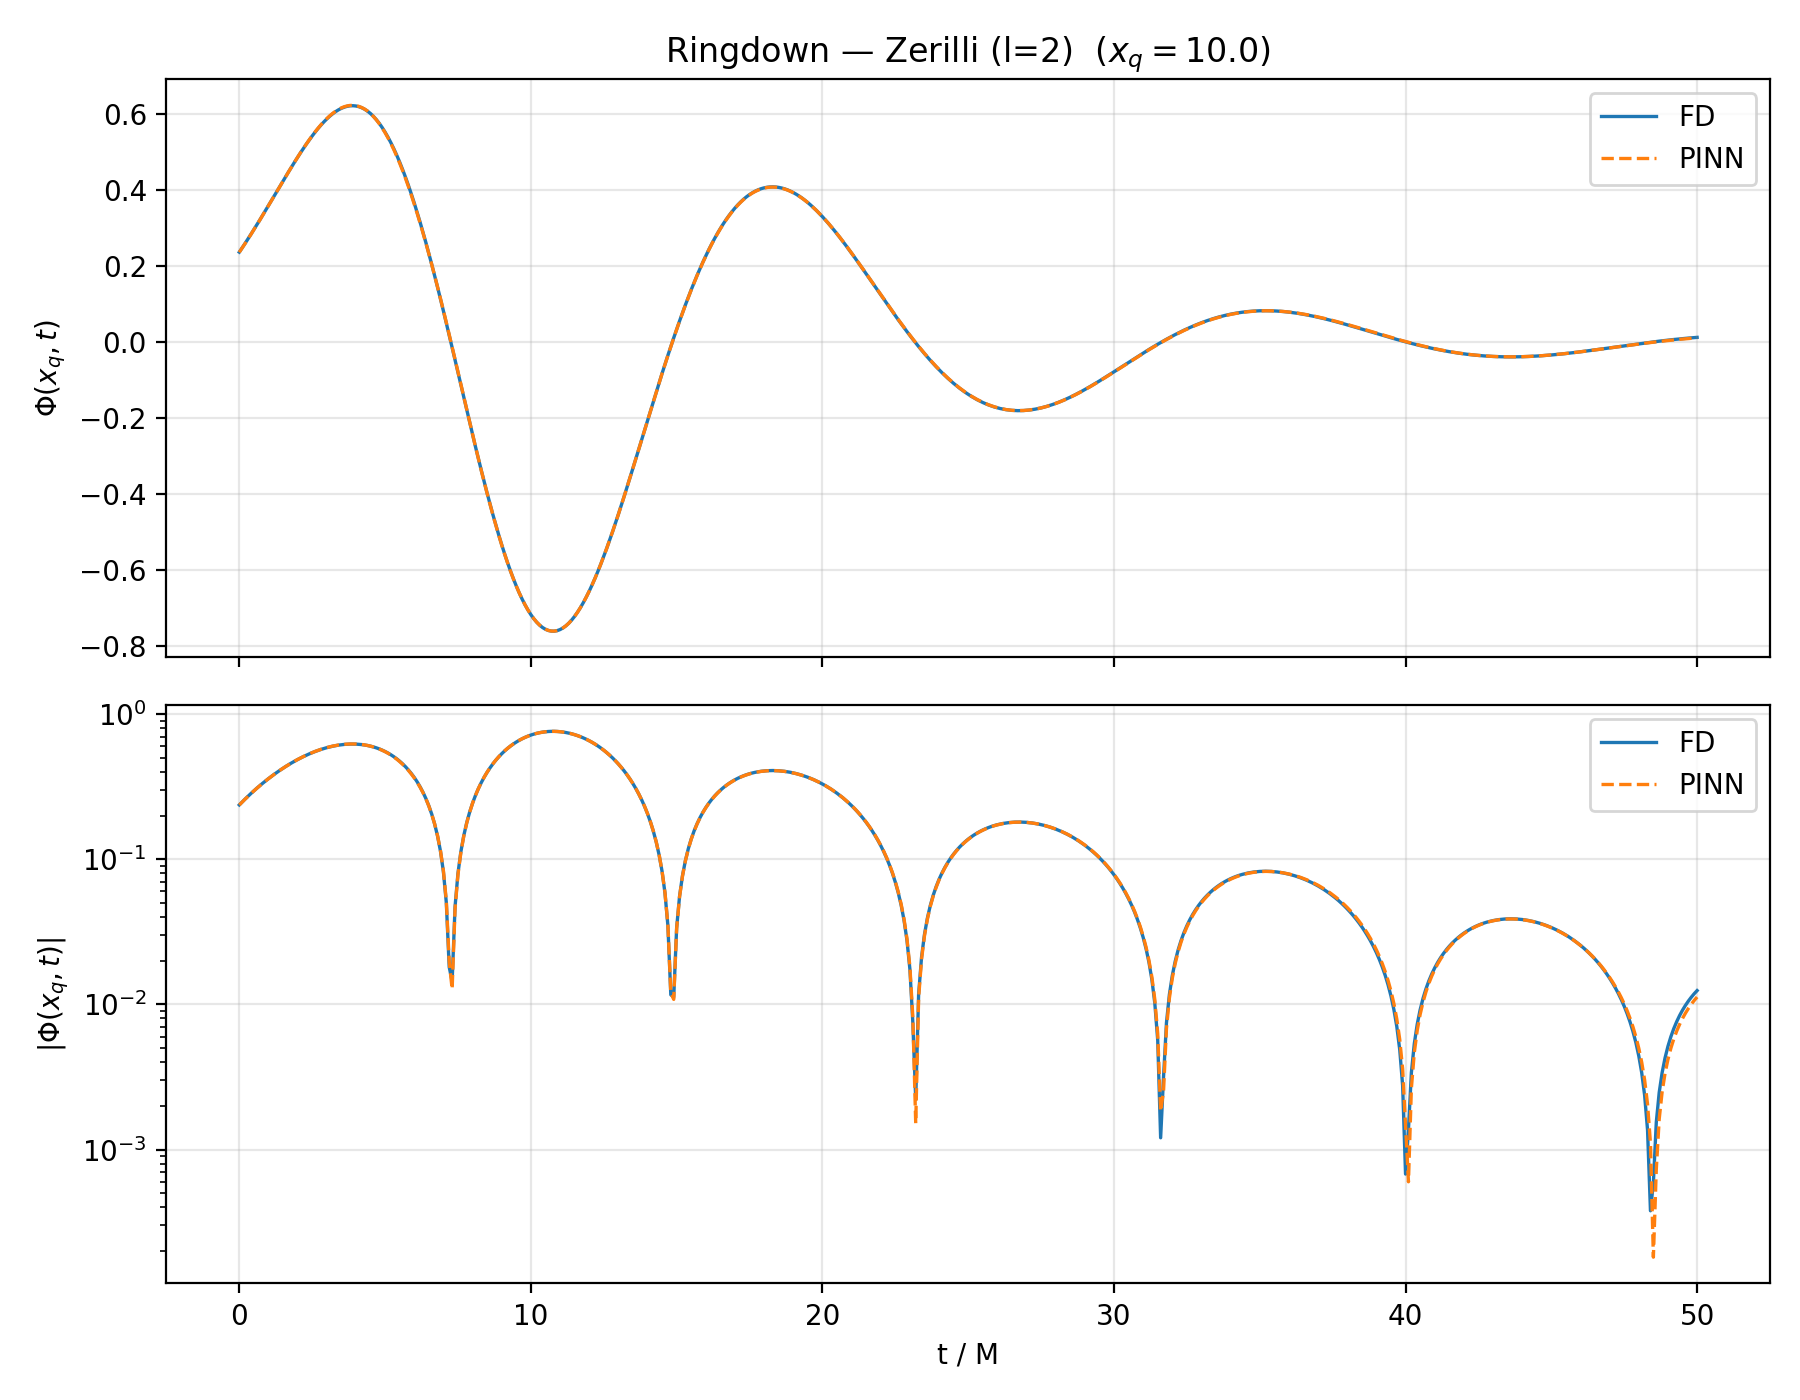
\includegraphics[width=\textwidth]{../outputs/pinn/zerilli_l2_greedy_f03_lbfgs30k/ringdown_overlay.png}
      \\{\footnotesize Ringdown waveform $\Phi(x_q\!=\!10M,\,t)$}
    \end{column}
  \end{columns}
\end{frame}

\begin{frame}{From Einstein's equations to a 1+1D wave problem}
  \textbf{Step 1 --- background.} Schwarzschild geometry ($M$ is the \bh{} mass),
  \[
    \mathrm{d} s^{2} \;=\; -f(r)\,\mathrm{d} t^{2} + f(r)^{-1}\mathrm{d} r^{2}
                     + r^{2}\,\mathrm{d}\Omega^{2},
    \qquad f(r) = 1 - \tfrac{2M}{r}.
  \]

  \textbf{Step 2 --- linear perturbation.} Write
  $g_{\mu\nu} = g^{(0)}_{\mu\nu} + h_{\mu\nu}$ with $|h| \ll |g^{(0)}|$ and
  expand the vacuum Einstein equations to first order:
  $\delta R_{\mu\nu}[h] = 0$.

  \textbf{Step 3 --- exploit spherical symmetry.} Decompose $h_{\mu\nu}$ in
  \emph{tensor spherical harmonics}; the modes split into two
  \textbf{decoupled parity sectors}:
  \medskip
  \begin{center}\small
  \begin{tabular}{lll}
    \toprule
    Sector & Parity & Master equation \\ \midrule
    \textbf{Axial} (odd) & $(-1)^{\ell+1}$ & \rw{} \\
    \textbf{Polar} (even)& $(-1)^{\ell}$   & \zer{} \\
    \bottomrule
  \end{tabular}
  \end{center}
  \medskip
  Each sector reduces to a single scalar field $\Phi(t,r_{\!*})$ on the
  \textbf{tortoise coordinate} $\mathrm{d} r_{\!*} = \mathrm{d} r/f(r)$.
\end{frame}

\begin{frame}{The two master equations --- \rw{} and \zer{}}
  Both sectors obey the \textbf{same 1+1D wave form}
  \[
    -\,\frac{\partial^{2}\Phi}{\partial t^{2}}
    \;+\; \frac{\partial^{2}\Phi}{\partial r_{\!*}^{\,2}}
    \;-\; V_{\ell}(r)\,\Phi \;=\; 0 ,
  \]
  but with two \emph{different} effective potentials:
  \medskip
  \begin{columns}[T]
    \begin{column}{0.42\textwidth}
      \centering\textbf{\rw{} (axial)}\par\medskip
      \[
        V^{\mathrm{RW}}_{\ell}(r) = f(r)\!\left[\frac{\ell(\ell{+}1)}{r^{2}} - \frac{6M}{r^{3}}\right]
      \]
    \end{column}
    \begin{column}{0.56\textwidth}
      \centering\textbf{\zer{} (polar)}\par\medskip
      \[
        V^{\mathrm{Z}}_{\ell}(r) = f(r)\,\frac{2\bigl[n^{2}(n{+}1)r^{3}+3n^{2}Mr^{2}+9nM^{2}r+9M^{3}\bigr]}{r^{3}(nr+3M)^{2}}
      \]
      {\centering\scriptsize $n = \tfrac{1}{2}(\ell-1)(\ell+2)$.\par}
    \end{column}
  \end{columns}
  \vfill
  \footnotesize
  Two \emph{different} potentials, one per parity sector --- but they encode
  \emph{the same physics}, as the next slide shows.
\end{frame}

\begin{frame}{Isospectrality --- one spectrum, two potentials}
  \begin{columns}[T]
    \begin{column}{0.55\textwidth}
      \centering
      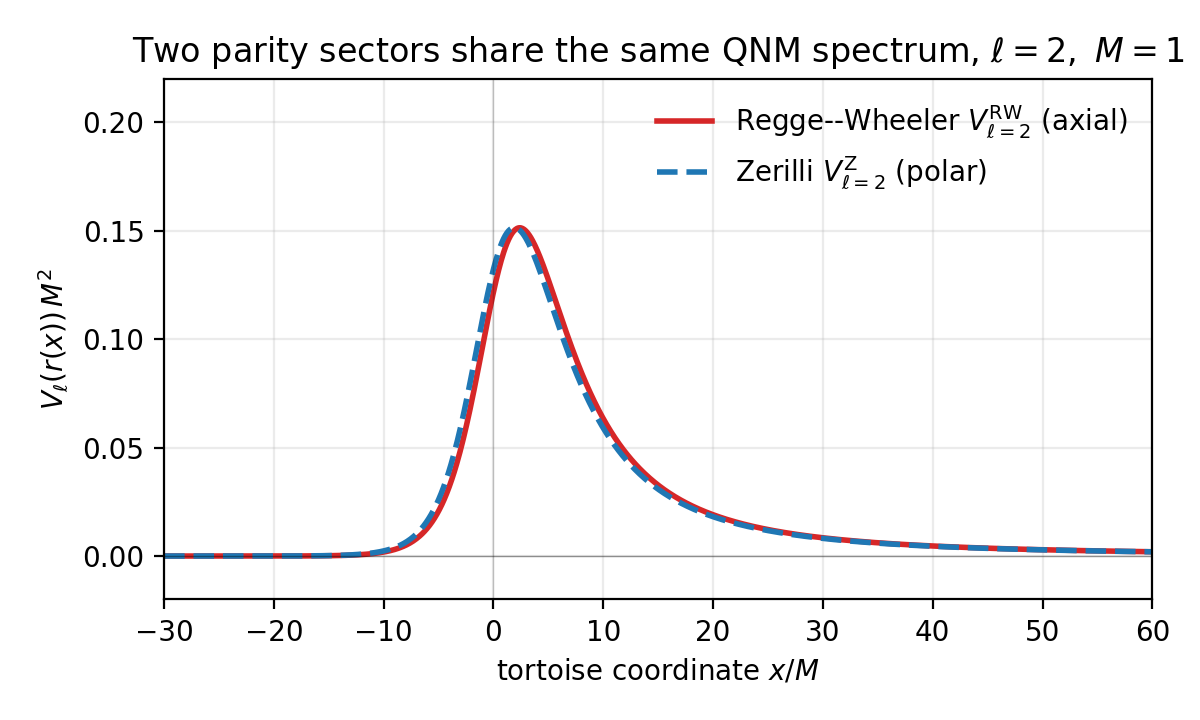
\includegraphics[width=\textwidth]{../outputs/background/rw_vs_zerilli_l2.png}
    \end{column}
    \begin{column}{0.43\textwidth}
      \footnotesize
      \textbf{Chandrasekhar--Detweiler isospectrality:} the two
      potentials are \emph{distinct} but share \emph{exactly the same}
      \qnm{} spectrum $\{\omega_{n}\}$.
      \medskip

      $\Rightarrow$ Either equation is a valid target for our solver.
      \medskip

      This work uses the \textbf{\zer{} (polar, $\ell\!=\!2$)} form,
      matching the reference PINN literature (Patel \emph{et al.}\ 2024)
      and giving a single, well-defined benchmark to push accuracy
      against.
    \end{column}
  \end{columns}
\end{frame}

\begin{frame}{The numerical problem we actually solve}
  Target: the polar $\ell\!=\!2$ \zer{} equation on
  $r_{\!*}/M \in [-50,\,150]$, $t/M \in [0,\,50]$.
  \medskip
  \begin{itemize}
    \item \textbf{Initial condition} ($t=0$): localised Gaussian pulse.
    \item \textbf{Boundary conditions:}
          \emph{purely outgoing} at $r_{\!*}\!\to\!+\infty$,
          \emph{purely ingoing} at $r_{\!*}\!\to\!-\infty$ (horizon).
    \item These BCs are precisely what selects the discrete
          \textbf{\qnm{} spectrum} $\omega_{n}\in\mathbb{C}$.
  \end{itemize}
  \medskip
  \textbf{Reference fundamental mode} ($\ell\!=\!2,\,n\!=\!0$, Leaver 1985):
  \[
    M\omega \;=\; 0.3737 - 0.0890\,i,
    \qquad \tau/M \;=\; -1/\Im\omega \;=\; 11.241 .
  \]
  Every result in this talk is benchmarked against this number.
\end{frame}

\begin{frame}{Three ways to compute \qnms{}}
  \footnotesize
  \begin{block}{1.\ Leaver continued fraction (1985) --- the \emph{exact reference}}
    Frobenius ansatz $\Rightarrow$ 3-term recurrence $\Rightarrow$ continued fraction.\;
    \textbf{+} 12-digit accuracy in ms.\quad
    \textbf{--} only known analytic potentials.
  \end{block}
  \begin{block}{2.\ Finite-difference (\fd{}) time evolution --- the \emph{ground-truth waveform}}
    2nd-order centred FD on the $(r_{\!*}, t)$ grid; extract $\omega,\tau$ from the
    late-time signal.\; \textbf{+} full $(x,t)$ field.\quad \textbf{--} \emph{expensive when accurate}.
  \end{block}
  \begin{block}{3.\ Neural solvers --- \emph{our tools}}
    \textbf{(a) \pinn{}:} mesh-free, differentiable solver for \emph{one} configuration.\\
    \textbf{(b) Hybrid \fno{}:} a cheap coarse FD solve $+$ a neural correction, trained
    \emph{once} over a \emph{family} of \bh{}s.
  \end{block}
\end{frame}

\begin{frame}{Why do we want a cheap, generalising solver?}
  \qnm{} extraction needs the \textbf{time-domain waveform} --- i.e.\ a PDE solve.
  Classical FD is accurate but its cost \emph{explodes} exactly where the science is:
  \medskip
  \begin{itemize}\small
    \item \textbf{High oscillation.} Higher multipoles $\ell$ and higher spin push the
          ringdown to \emph{shorter wavelengths}; resolving them forces a finer grid,
          and FD cost scales as $\sim\!k^{\,d+1}$ in the refinement factor $k$.
    \item \textbf{High dimension.} Schwarzschild is $1{+}1$D; Kerr (Teukolsky) is
          $2{+}1$D. Each added dimension multiplies the grid cost.
    \item \textbf{Many-query regimes.} Parameter estimation, population studies and
          surrogate building need \emph{thousands} of solves over $(M, a, \text{initial data})$.
  \end{itemize}
  \medskip
  \begin{block}{\footnotesize The two neural answers in this talk}
    \footnotesize
    \textbf{\pinn{}} --- a \emph{differentiable} mesh-free solver: a single trained
    network, but \emph{one solve per configuration}.\\[2pt]
    \textbf{Hybrid \fno{}} --- keep a \emph{cheap} coarse solver as the workhorse and
    learn only the part it cannot resolve, \emph{amortised} over a whole parameter
    family with a single forward pass per new \bh{}.
  \end{block}
\end{frame}

\begin{frame}{What this project contributes}
  Schwarzschild $\ell\!=\!2$ is the \textbf{stress test} for \qnm{} surrogates ---
  every error is measurable against an exact reference.
  \medskip
  \begin{enumerate}
    \item \textbf{Forward PINN, accuracy push:} hard BCs, gPINN residuals,
          \textbf{greedy adaptive sampling}, extended L-BFGS.
          Field error to \textbf{0.58\%} (Patel: $28\%$, a $\sim\!50\times$ reduction)
          and $\omega$ to \textbf{0.03\%} (M4).
    \medskip
    \item \textbf{New extraction methodology --- M1--M5:} from FFT/NLS to
          ESPRIT and \emph{plateau scans} that give principled, falsifiable
          $(\omega,\tau)$ with systematic-error bars.
    \medskip
    \item \textbf{Hybrid coarse-FD $+$ neural-residual surrogate:} a
          \emph{label-free}, \emph{gated} \fno{} that super-resolves a cheap
          $k\!=\!4$ coarse solve by $\sim\!10\times$ in field error, generalising
          across a $1000$-\bh{} family at $1/64$ of the fine-FD cost.
  \end{enumerate}
  \medskip
  \footnotesize This talk presents our \textbf{best forward PINN} and the
  \textbf{hybrid FNO}, and compares both against the reference paper.
\end{frame}


% ══════════════════════════════════════════════════════════════════
\section{2. PINN Methodology}
% ══════════════════════════════════════════════════════════════════

\begin{frame}{Forward PINN --- problem statement}
  \textbf{Goal.} Train a network $\Phi_{\boldsymbol{\theta}}(x,t)$ to satisfy the
  \zer{} PDE on the full $(x,t)$ domain, plus its initial and boundary conditions.
  \bigskip

  We minimise a sum of \textbf{seven} weighted mean-squared-error terms,
  \[
    \mathcal{L}_{\text{fwd}}(\boldsymbol{\theta})
    =
    \underbrace{\textcolor{darkred}{\lambda_{r}\mathcal{L}_{r}
      + \lambda_{r_x}\mathcal{L}_{r_x}
      + \lambda_{r_t}\mathcal{L}_{r_t}}}_{\text{PDE residual + gPINN}}
    +
    \underbrace{\textcolor{darkgreen}{\lambda_{ic}\mathcal{L}_{ic}
      + \lambda_{iv}\mathcal{L}_{iv}}}_{\text{initial condition}}
    +
    \underbrace{\textcolor{blue}{\lambda_{bl}\mathcal{L}_{bl}
      + \lambda_{br}\mathcal{L}_{br}}}_{\text{boundary conditions}}
  \]
  \bigskip
  Each $\mathcal{L}_i$ is a mean of squared residuals over a sample of
  collocation points; the next two slides write the seven sums explicitly.
\end{frame}

\begin{frame}{Forward PINN loss --- PDE residual $+$ gPINN}
  \footnotesize
  \textbf{PDE residual} of the \zer{} equation,
  \[
    r_{\theta}(x,t) \equiv
    -\,\partial_{t}^{2}\Phi_{\theta}
    + \partial_{x}^{2}\Phi_{\theta}
    - V_{\ell}(r)\,\Phi_{\theta}.
  \]
  At $N_{r}=32{,}000$ collocation points we evaluate
  \[
    \textcolor{darkred}{\mathcal{L}_{r}}
      = \tfrac{1}{N_{r}}\!\sum_{i}\!\bigl[r_{\theta}(x_{i},t_{i})\bigr]^{2}
    \quad\text{(standard PINN residual),}
  \]
  \[
    \textcolor{darkred}{\mathcal{L}_{r_{x}}}
      = \tfrac{1}{N_{r}}\!\sum_{i}\!\bigl[\partial_{x} r_{\theta}\bigr]^{2},
    \qquad
    \textcolor{darkred}{\mathcal{L}_{r_{t}}}
      = \tfrac{1}{N_{r}}\!\sum_{i}\!\bigl[\partial_{t} r_{\theta}\bigr]^{2}.
  \]
  \medskip
  The two extra terms are the \textbf{gPINN} regularisers (Yu \emph{et al.}\ 2022):
  penalising the \emph{gradient} of the residual forces it to be smoothly small,
  not just point-wise small, and gives noticeably cleaner derivatives.
\end{frame}

\begin{frame}{Forward PINN loss --- initial and boundary conditions}
  \footnotesize
  \textcolor{darkgreen}{\textbf{Initial condition} at $t=0$} on $N_{\mathrm{ic}}$ spatial points:
  \[
    \textcolor{darkgreen}{\mathcal{L}_{\mathrm{ic}}}
      = \tfrac{1}{N_{\mathrm{ic}}}\!\sum_{j}\!\bigl[\Phi_{\theta}(x_{j},0)-\Phi_{0}(x_{j})\bigr]^{2}
    \;\;(\Phi_{0}\text{ a Gaussian pulse}),
  \]
  \[
    \textcolor{darkgreen}{\mathcal{L}_{\mathrm{iv}}}
      = \tfrac{1}{N_{\mathrm{ic}}}\!\sum_{j}\!\bigl[\partial_{t}\Phi_{\theta}(x_{j},0)\bigr]^{2}
    \quad\text{(time-symmetric data)}.
  \]
  \medskip
  \textcolor{blue}{\textbf{Boundary conditions}} on $N_{\mathrm{bc}}$ time points ---
  outgoing at $x_{\max}$, ingoing at $x_{\min}$:
  \[
    \textcolor{blue}{\mathcal{L}_{\mathrm{bl}}}
      = \tfrac{1}{N_{\mathrm{bc}}}\!\sum_{k}\!\bigl[(\partial_{t}-\partial_{x})\Phi_{\theta}(x_{\min},t_{k})\bigr]^{2},
  \]
  \[
    \textcolor{blue}{\mathcal{L}_{\mathrm{br}}}
      = \tfrac{1}{N_{\mathrm{bc}}}\!\sum_{k}\!\bigl[(\partial_{t}+\partial_{x})\Phi_{\theta}(x_{\max},t_{k})\bigr]^{2}.
  \]
\end{frame}

\begin{frame}{Forward PINN --- training setup}
  \begin{itemize}
    \item \textbf{Network.} Fully-connected MLP, widths
          $[\,2,80,40,20,10,1\,]$, $\tanh$ ($\sim\!4{,}500$ params).
    \item \textbf{Output transform.}
          $\Phi_{\theta}=A\tanh(\widetilde{\Phi}_{\theta})$, $A=1$ ---
          bounds the field, stabilises early training.
    \item \textbf{Loss weights.}
          $\boldsymbol{\lambda} = (100,100,100,\,1,100,\,1,1)$.
    \item \textbf{Optimiser.} Adam for $10{,}000$ steps to find a basin, then
          \textbf{L-BFGS} for $30{,}000$ steps to converge inside it.
    \item \textbf{Sampling.} Collocation points re-drawn every epoch via
          \emph{greedy resampling} (next three slides) --- our key training
          innovation.
  \end{itemize}
\end{frame}

\begin{frame}{Forward PINN --- architecture}
  \centering
  \resizebox{0.95\textwidth}{!}{%
  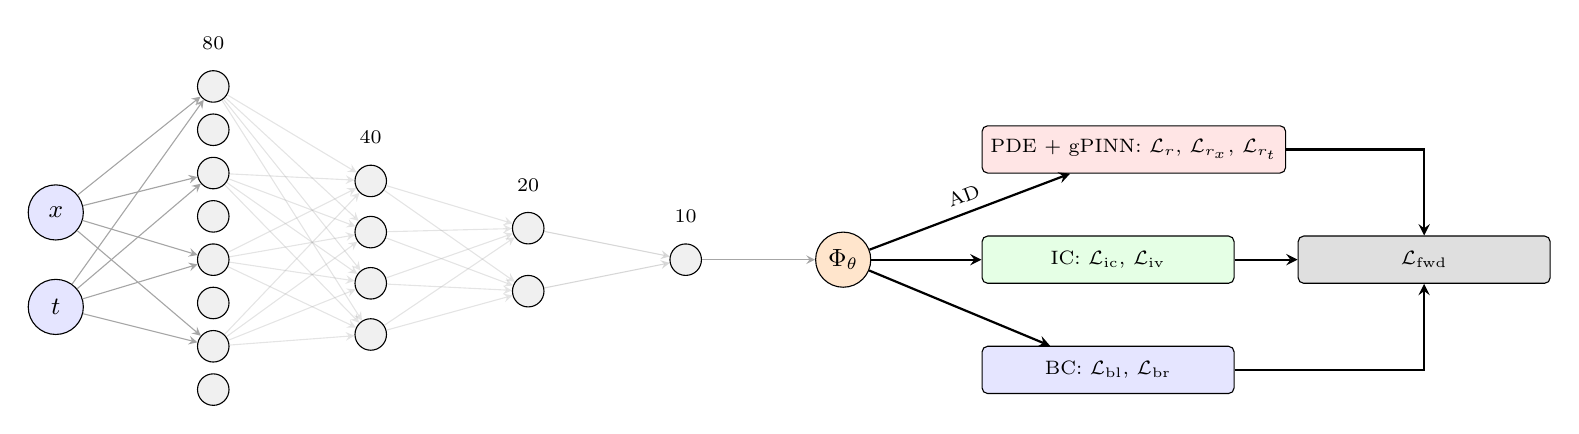
\begin{tikzpicture}[
    node distance=10mm and 12mm,
    every node/.style={font=\small},
    inp/.style={circle, draw, fill=blue!10, minimum size=7mm, inner sep=0pt},
    hid/.style={circle, draw, fill=gray!12, minimum size=4mm, inner sep=0pt},
    outn/.style={circle, draw, fill=orange!20, minimum size=7mm, inner sep=0pt},
    loss/.style={rectangle, draw, fill=green!10, rounded corners=2pt,
                 minimum height=6mm, minimum width=32mm, inner sep=3pt,
                 align=center, font=\scriptsize},
    arr/.style={->, >=stealth, thin, gray!70},
  ]
    \node[inp] (x) at (0, 0) {$x$};
    \node[inp] (t) at (0, -1.2) {$t$};
    \def\xL{2.0}\def\xLii{4.0}\def\xLiii{6.0}\def\xLiv{8.0}
    \foreach \k/\y in {1/1.6, 2/1.05, 3/0.5, 4/-0.05, 5/-0.6, 6/-1.15, 7/-1.7, 8/-2.25}{
      \node[hid] (a\k) at (\xL, \y) {};}
    \foreach \k/\y in {1/0.4, 2/-0.25, 3/-0.9, 4/-1.55}{
      \node[hid] (b\k) at (\xLii, \y) {};}
    \foreach \k/\y in {1/-0.2, 2/-1.0}{
      \node[hid] (c\k) at (\xLiii, \y) {};}
    \node[hid] (d1) at (\xLiv, -0.6) {};
    \node[font=\scriptsize] at (\xL, 2.15) {$80$};
    \node[font=\scriptsize] at (\xLii, 0.95) {$40$};
    \node[font=\scriptsize] at (\xLiii, 0.35) {$20$};
    \node[font=\scriptsize] at (\xLiv, -0.05) {$10$};
    \node[outn] (phi) at (10.0, -0.6) {$\Phi_\theta$};
    \foreach \src in {x, t}\foreach \dst in {a1, a3, a5, a7}\draw[arr] (\src) -- (\dst);
    \foreach \a in {1,3,5,7}\foreach \b in {1,2,3,4}\draw[arr, opacity=0.30] (a\a) -- (b\b);
    \foreach \a in {1,2,3,4}\foreach \b in {1,2}\draw[arr, opacity=0.30] (b\a) -- (c\b);
    \foreach \a in {1,2}\draw[arr, opacity=0.45] (c\a) -- (d1);
    \draw[arr] (d1) -- (phi);
    \node[loss, fill=red!10, right=14mm of phi, yshift=14mm] (lpde)
      {PDE + gPINN: $\mathcal{L}_{r},\,\mathcal{L}_{r_x},\,\mathcal{L}_{r_t}$};
    \node[loss, fill=green!10, right=14mm of phi] (lic)
      {IC: $\mathcal{L}_{\mathrm{ic}},\,\mathcal{L}_{\mathrm{iv}}$};
    \node[loss, fill=blue!10, right=14mm of phi, yshift=-14mm] (lbc)
      {BC: $\mathcal{L}_{\mathrm{bl}},\,\mathcal{L}_{\mathrm{br}}$};
    \draw[arr, thick, black] (phi) -- (lpde) node[midway, above, font=\scriptsize, sloped] {AD};
    \draw[arr, thick, black] (phi) -- (lic);
    \draw[arr, thick, black] (phi) -- (lbc);
    \node[loss, fill=gray!25, right=8mm of lic] (ltot)
      {$\mathcal{L}_{\mathrm{fwd}}$};
    \draw[arr, thick, black] (lpde) -| (ltot);
    \draw[arr, thick, black] (lic) -- (ltot);
    \draw[arr, thick, black] (lbc) -| (ltot);
  \end{tikzpicture}}
  \\[6pt]
  \begin{minipage}{0.92\textwidth}
    \centering\scriptsize
    Inputs $(x,t)$ feed a four-layer $\tanh$ MLP ($80\!\to\!40\!\to\!20\!\to\!10$,
    $\sim\!4{,}500$ params); the output passes through
    $\Phi_{\theta}=A\tanh(\widetilde{\Phi}_{\theta})$ and is differentiated by
    automatic differentiation (\textbf{AD}) to form the seven residuals.
  \end{minipage}
\end{frame}

\begin{frame}{Innovation --- why adaptive sampling matters}
  \begin{columns}[T]
    \begin{column}{0.50\textwidth}
      Uniform collocation wastes points where the residual is already small and
      starves the network where it is large.
      \medskip
      \begin{itemize}\small
        \item \textbf{Residual-Adaptive Distribution (RAD)}
              [Wu \emph{et al.}\ 2023]: probabilistic resampling
              $p_{i}\propto|r_{i}|^{k}+c$. Two hyperparameters.
        \item Stochastic $\Rightarrow$ extreme residuals not always selected.
        \item Sampling noise can interfere with Adam dynamics.
      \end{itemize}
    \end{column}
    \begin{column}{0.48\textwidth}
      \centering
      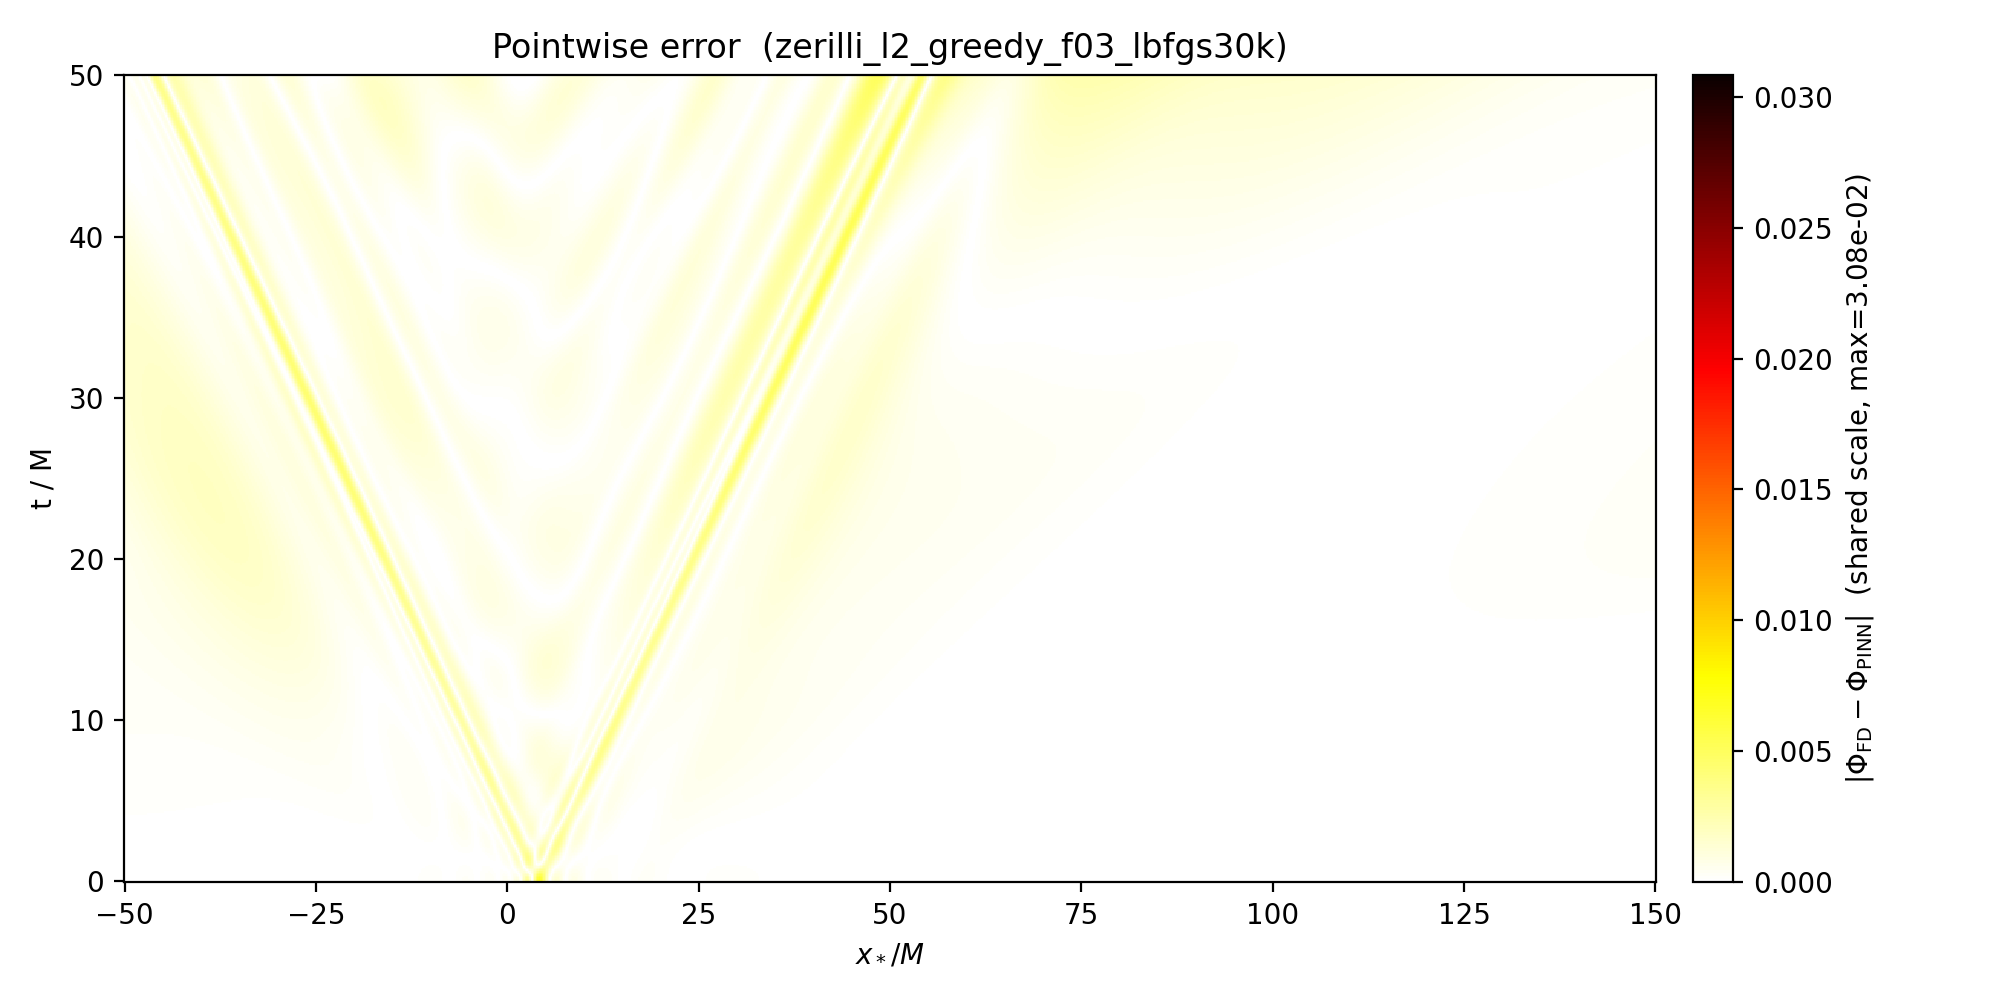
\includegraphics[width=\textwidth]{../outputs/pinn/zerilli_l2_greedy_f03_lbfgs30k/error_heatmap.png}
      \\{\footnotesize Final error map: residual concentrates along the
      wavefronts travelling out from the burst.}
    \end{column}
  \end{columns}
\end{frame}

\begin{frame}{Innovation --- greedy resampling algorithm}
  Replace probabilistic RAD with \textbf{deterministic top-$N$} selection:
  \medskip
  \begin{enumerate}\small
    \item Every $P$ Adam steps, generate $N_{\text{cand}}\!=\!100{,}000$ random
          candidates in the domain.
    \item Evaluate the PDE residual $|r_{i}|$ at each (one batched forward pass).
    \item \textbf{Sort by $|r_{i}|$ descending}; keep the top $f\!\cdot\!N_{r}$.
    \item Fill the remaining $(1{-}f)N_{r}$ slots with \textbf{uniform random}
          points (preserves exploration).
    \item Replace all $N_{r}\!=\!32{,}000$ collocation points; continue Adam.
  \end{enumerate}
  \medskip
  \textbf{Advantages over RAD:} \emph{deterministic} (worst residuals always kept);
  a \emph{single} hyperparameter $f$ ($0$ = uniform, $1$ = fully greedy); no
  $|r|^{k}+c$ shape to tune.
\end{frame}

\begin{frame}{Innovation --- greedy $f$ sweep}
  \begin{columns}[T]
    \begin{column}{0.50\textwidth}
      \centering\footnotesize
      \begin{tabular}{@{}lcc@{}}
        \toprule
        \textbf{Configuration} & \textbf{RMSD} & \textbf{vs.\ base} \\
        \midrule
        Uniform (baseline)  & 0.00183 & --- \\
        RAD $k\!=\!2$       & 0.00095 & $-48\%$ \\
        \midrule
        Greedy $f\!=\!0.3$  & \textbf{0.00085} & \textbf{$-54\%$} \\
        Greedy $f\!=\!0.5$  & 0.00107 & $-42\%$ \\
        Greedy $f\!=\!0.8$  & 0.00165 & $-10\%$ \\
        \rowcolor{green!10}
        Greedy $f\!=\!0.3$ + L-BFGS 30k & \textbf{0.00082} & \textbf{$-55\%$} \\
        \bottomrule
      \end{tabular}
    \end{column}
    \begin{column}{0.48\textwidth}
      \begin{itemize}\small
        \item \textbf{$f\!=\!0.3$ optimal:} 30\% greedy + 70\% uniform balances
              exploitation and exploration.
        \item Too aggressive ($f\!\ge\!0.5$): network over-fits the high-residual
              band and regresses elsewhere.
        \item \textbf{Beats RAD with a simpler, deterministic, one-knob algorithm.}
        \item Combined with extended L-BFGS $\Rightarrow$ our best forward PINN.
      \end{itemize}
    \end{column}
  \end{columns}
\end{frame}


% ══════════════════════════════════════════════════════════════════
\section{3. QNM Extractors (M1--M5)}
% ══════════════════════════════════════════════════════════════════

\begin{frame}{QNM Extraction Methods}
  Every solver (PINN, hybrid FNO, FD) outputs a waveform $\Phi(\xq,t)$; the \qnm{}
  is then \emph{extracted}. We report \textbf{five} methods and quote the best per quantity.
  \medskip
  \begin{itemize}\small
    \item \textbf{M1 --- FFT $+$ log-linear envelope:} $\omega$ from the FFT peak,
          $\tau$ from the $\log|\text{peaks}|$ slope. Fast, but single-window.
    \item \textbf{M2 --- single-mode NLS:} fit $A e^{-t/\tau}\cos(\omega t+\phi)$ over a
          window. Best wide-window $\tau$ estimator; biased by overtones early.
    \item \textbf{M3 --- ESPRIT}, \textbf{M4 --- 1-D plateau scan},
          \textbf{M5 --- 2-D plateau scan} are detailed on the next slides.
  \end{itemize}
  \medskip
  \textbf{Two problems M1/M2 alone cannot solve:}
  \emph{overtone contamination} ($\tau_{1}\!\approx\!3.65M$ near the burst) and
  \emph{window dependence} (a single number with no sensitivity $\Rightarrow$ not falsifiable).
\end{frame}

\begin{frame}{M3 --- ESPRIT subspace decomposition}
  \textbf{Idea:} model the uniformly-sampled ringdown as a sum of $K$ complex
  exponentials (poles) and recover them \emph{simultaneously} by a subspace
  rotation --- no nonlinear fit and no initial guess (Estimation of Signal
  Parameters via Rotational Invariance Techniques).
  \[
    \Phi(\xq,\,k\Delta t)\;\approx\;\sum_{n=0}^{K-1} c_{n}\,z_{n}^{\,k},
    \qquad
    z_{n}=e^{(-1/\tau_{n}+i\omega_{n})\,\Delta t}.
  \]
  \textbf{Procedure:}
  \begin{enumerate}\small
    \item Hilbert-transform the real signal to its analytic form, so each
          physical mode appears once.
    \item Build the Hankel data matrix from the samples; SVD $\to$ signal
          subspace $\mathbf{U}$.
    \item Solve the rotational-invariance eigenproblem
          $\mathbf{U}_{1}^{\dagger}\mathbf{U}_{2}=\boldsymbol{\Psi}$; the poles are
          $z_{n}=\mathrm{eig}(\boldsymbol{\Psi})$.
    \item Read off $\omega_{n}=\Im(\log z_{n})/\Delta t$,\;
          $\tau_{n}=-\Delta t/\Re(\log z_{n})$; report the largest-amplitude mode.
  \end{enumerate}
  \medskip
  \textbf{Strength:} no initial guess; resolves multiple modes naturally.\quad
  \textbf{Weakness:} Hankel conditioning degrades on a clean single-mode tail, so
  on our QNM-dominated fields ESPRIT can return spurious machine-noise poles.
\end{frame}

\begin{frame}{M4 --- two-mode NLS with start-time plateau scan}
  \textbf{Step 1.} Fit a \emph{two-mode} template (fundamental + first overtone):
  \[
    \Phi_{\text{model}}(t)=
    A_{0}e^{-t/\tau_{0}}\cos(\omega_{0}t+\phi_{0})
    + A_{1}e^{-t/\tau_{1}}\cos(\omega_{1}t+\phi_{1})
  \]
  on $[t_{0},t_{\max}]$; identify the longer-$\tau$ mode as the fundamental.
  \medskip

  \textbf{Step 2.} Repeat over start times $t_{0}\in[10,25]M$; find the contiguous
  \textbf{plateau} of low-scatter consecutive fits.
  \medskip

  \textbf{Step 3.} Report
  $\omega_{\!_{M4}}=\langle\omega\rangle_{\text{plateau}}$,
  $\sigma_{\omega}=\mathrm{std}(\omega)_{\text{plateau}}$ ---
  the plateau spread is a \textbf{principled systematic error bar}.
  \medskip

  \footnotesize An honest extraction must be invariant to small window shifts;
  the plateau is the empirical signature of that invariance.
\end{frame}

\begin{frame}{M4 --- example stability scan}
  \begin{columns}[T]
    \begin{column}{0.52\textwidth}
      \centering
      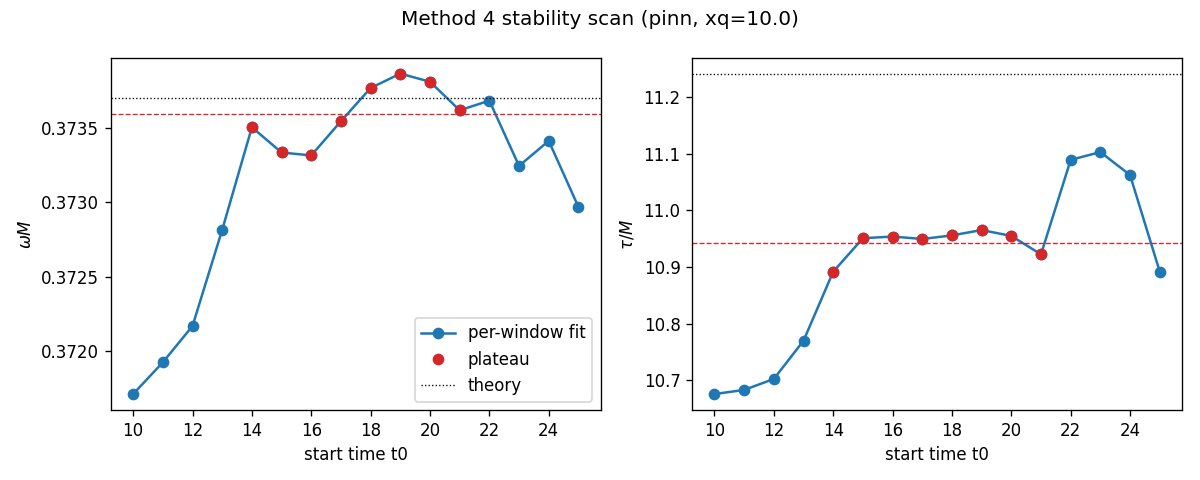
\includegraphics[width=\textwidth,height=0.78\textheight,keepaspectratio]{../outputs/qnm/zerilli_l2_greedy_f03_lbfgs30k/pinn_method4_stability.png}
      \\{\footnotesize Forward PINN: M4 stability scan over $t_{0}\in[10,25]M$.}
    \end{column}
    \begin{column}{0.46\textwidth}
      \begin{itemize}\small
        \item $\omega$ (top): flat across $t_{0}\in[14,21]M$ $\Rightarrow$ plateau.
        \item $\tau$ (bottom): stabilises once $t_{0}$ is past the prompt burst.
        \item Plateau quote
              $\omega_{\!_{M4}}=0.37359\pm1.96\!\times\!10^{-4}$
              $\Rightarrow$ \textbf{0.029\%} error.
        \item Green band $=2\sigma_{\omega}$: an honest, falsifiable systematic.
      \end{itemize}
    \end{column}
  \end{columns}
\end{frame}

\begin{frame}{M5 --- two-mode NLS with 2-D plateau scan}
  M4 sweeps only one window edge ($t_{0}$). \textbf{M5} sweeps both:
  \[
    [t_{0},t_{\text{end}}]\in[10,25]M\times[t_{\min},50]M
    \quad\text{on a }10\!\times\!6\text{ grid,}
  \]
  reporting the mean/stddev over the rectangular plateau of smallest joint scatter.
  \medskip
  \begin{itemize}\small
    \item $t_{0}$ scans control \emph{overtone leakage} (early edge).
    \item $t_{\text{end}}$ scans control \emph{Price-tail leakage} (late edge).
    \item Truncating either edge prematurely is a \emph{model-misspecification}
          bias --- it does \emph{not} vanish with more data.
    \item To our knowledge the \textbf{first systematic 2-D plateau analysis}
          for neural-solver ringdowns.
  \end{itemize}
\end{frame}

\begin{frame}{M5 --- example 2-D heatmap}
  \begin{columns}[T]
    \begin{column}{0.46\textwidth}
      \centering
      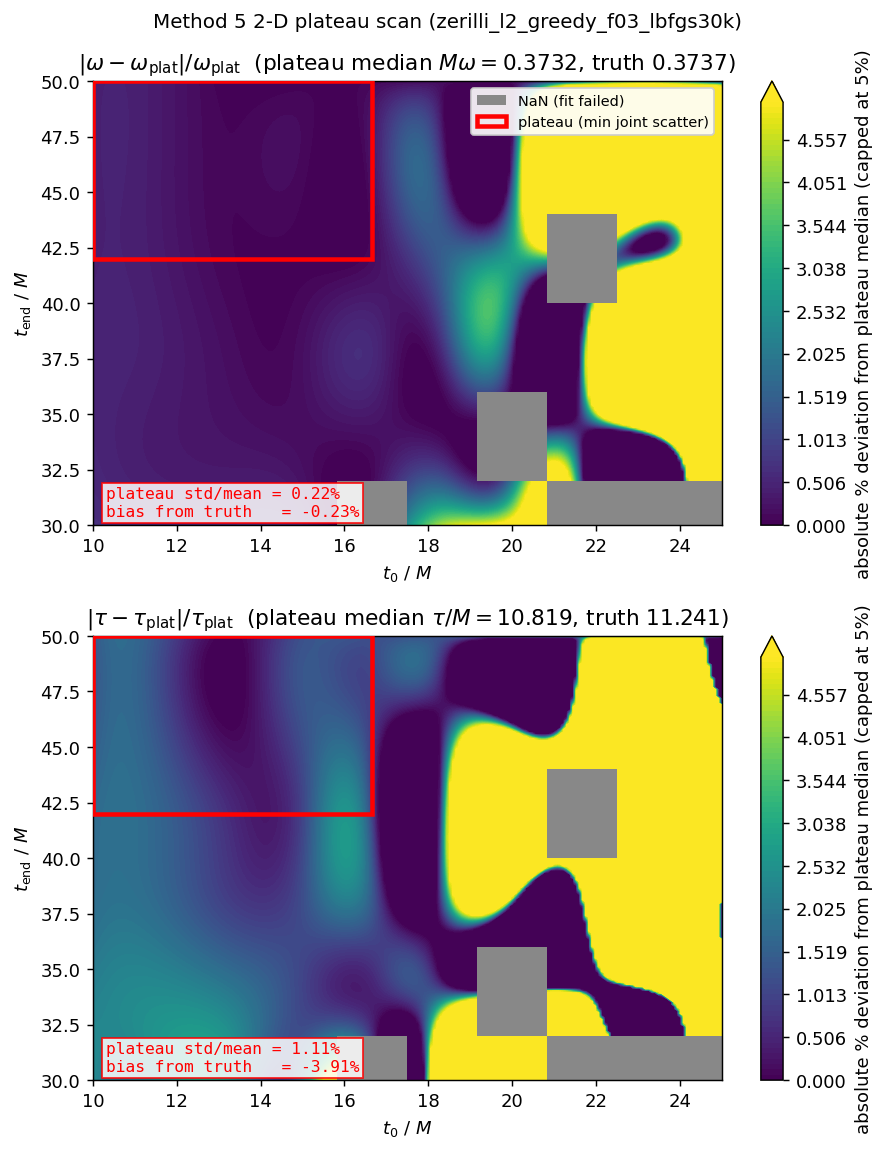
\includegraphics[width=\textwidth,height=0.80\textheight,keepaspectratio]{../outputs/qnm/zerilli_l2_greedy_f03_lbfgs30k/pinn_method5_2d_heatmap.png}
    \end{column}
    \begin{column}{0.52\textwidth}
      \footnotesize
      \textbf{Top:} $\omega$ map. \textbf{Bottom:} $\tau$ map.
      \begin{itemize}
        \item Axes: $t_{0}$ (start) vs $t_{\text{end}}$ (end).
        \item Colour: local relative scatter (capped $5\%$).
        \item \textcolor{red!75!black}{\textbf{Red box:}} plateau (minimum scatter).
        \item Grey: NaN cells where the two-mode fit failed.
      \end{itemize}
      \medskip
      \textbf{Plateau quote:}
      $\omega_{\!_{M5}}=0.3732$ ($0.13\%$),
      $\tau_{\!_{M5}}=10.82$ ($3.91\%$).
      M5 reproduces M4 \emph{and} certifies the right-edge choice is harmless.
    \end{column}
  \end{columns}
\end{frame}

\begin{frame}{Reporting convention --- best estimator per quantity}
  Different quantities are best estimated from different features of the waveform,
  so we quote a \textbf{best-per-quantity headline} (and list all five as cross-checks):
  \medskip
  \begin{center}\small
    \begin{tabular}{@{}lll@{}}
      \toprule
      \textbf{Quantity} & \textbf{Estimator} & \textbf{Reason} \\
      \midrule
      $\omega$ & \textbf{M4 / M5 plateau} &
        phase aggregated across cycles; lowest variance. \\
      \addlinespace
      $\tau$ & \textbf{M2 wide window} or \textbf{M4/M5 plateau} &
        amplitude over the longest clean decay range. \\
      \bottomrule
    \end{tabular}
  \end{center}
  \medskip
  \begin{itemize}\small
    \item Consistent with NR ringdown practice (Berti \emph{et al.}\ 2007).
    \item Patel \emph{et al.}\ 2024 use a similar split but report
          \emph{no} fit-window sensitivity.
    \item \textbf{From here on, every result quotes field error $+$ the best
          M1--M5 fit for $\omega$ and $\tau$, naming the extractor.}
  \end{itemize}
\end{frame}


% ══════════════════════════════════════════════════════════════════
\section{4. PINN Results}
% ══════════════════════════════════════════════════════════════════

\begin{frame}{Forward PINN --- waveform agreement}
  \centering
  \begin{columns}[T]
    \begin{column}{0.50\textwidth}
      \centering
      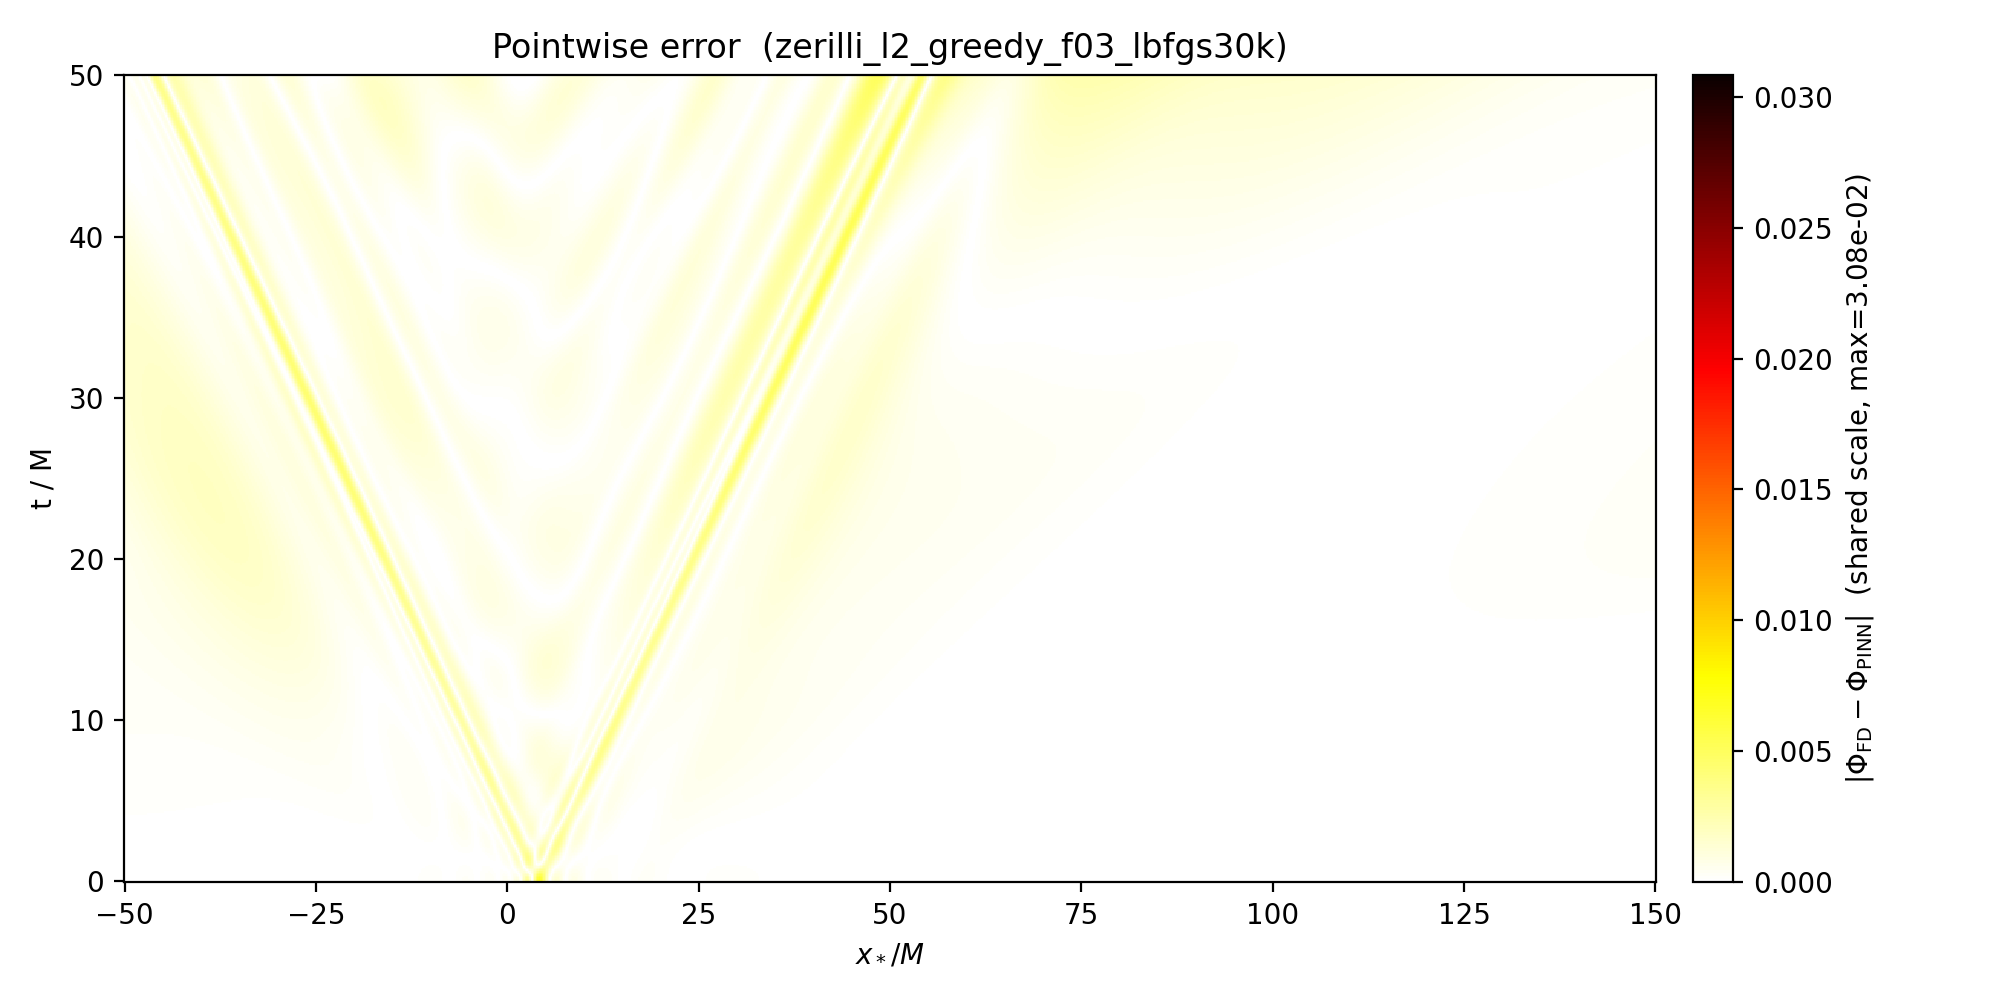
\includegraphics[width=\linewidth,height=0.70\textheight,keepaspectratio]{../outputs/pinn/zerilli_l2_greedy_f03_lbfgs30k/error_heatmap.png}
      \\[3pt]{\scriptsize Pointwise error $|\Phi_{\pinn{}}-\Phi_{\fd{}}|$ over the full domain.}
    \end{column}
    \begin{column}{0.48\textwidth}
      \centering
      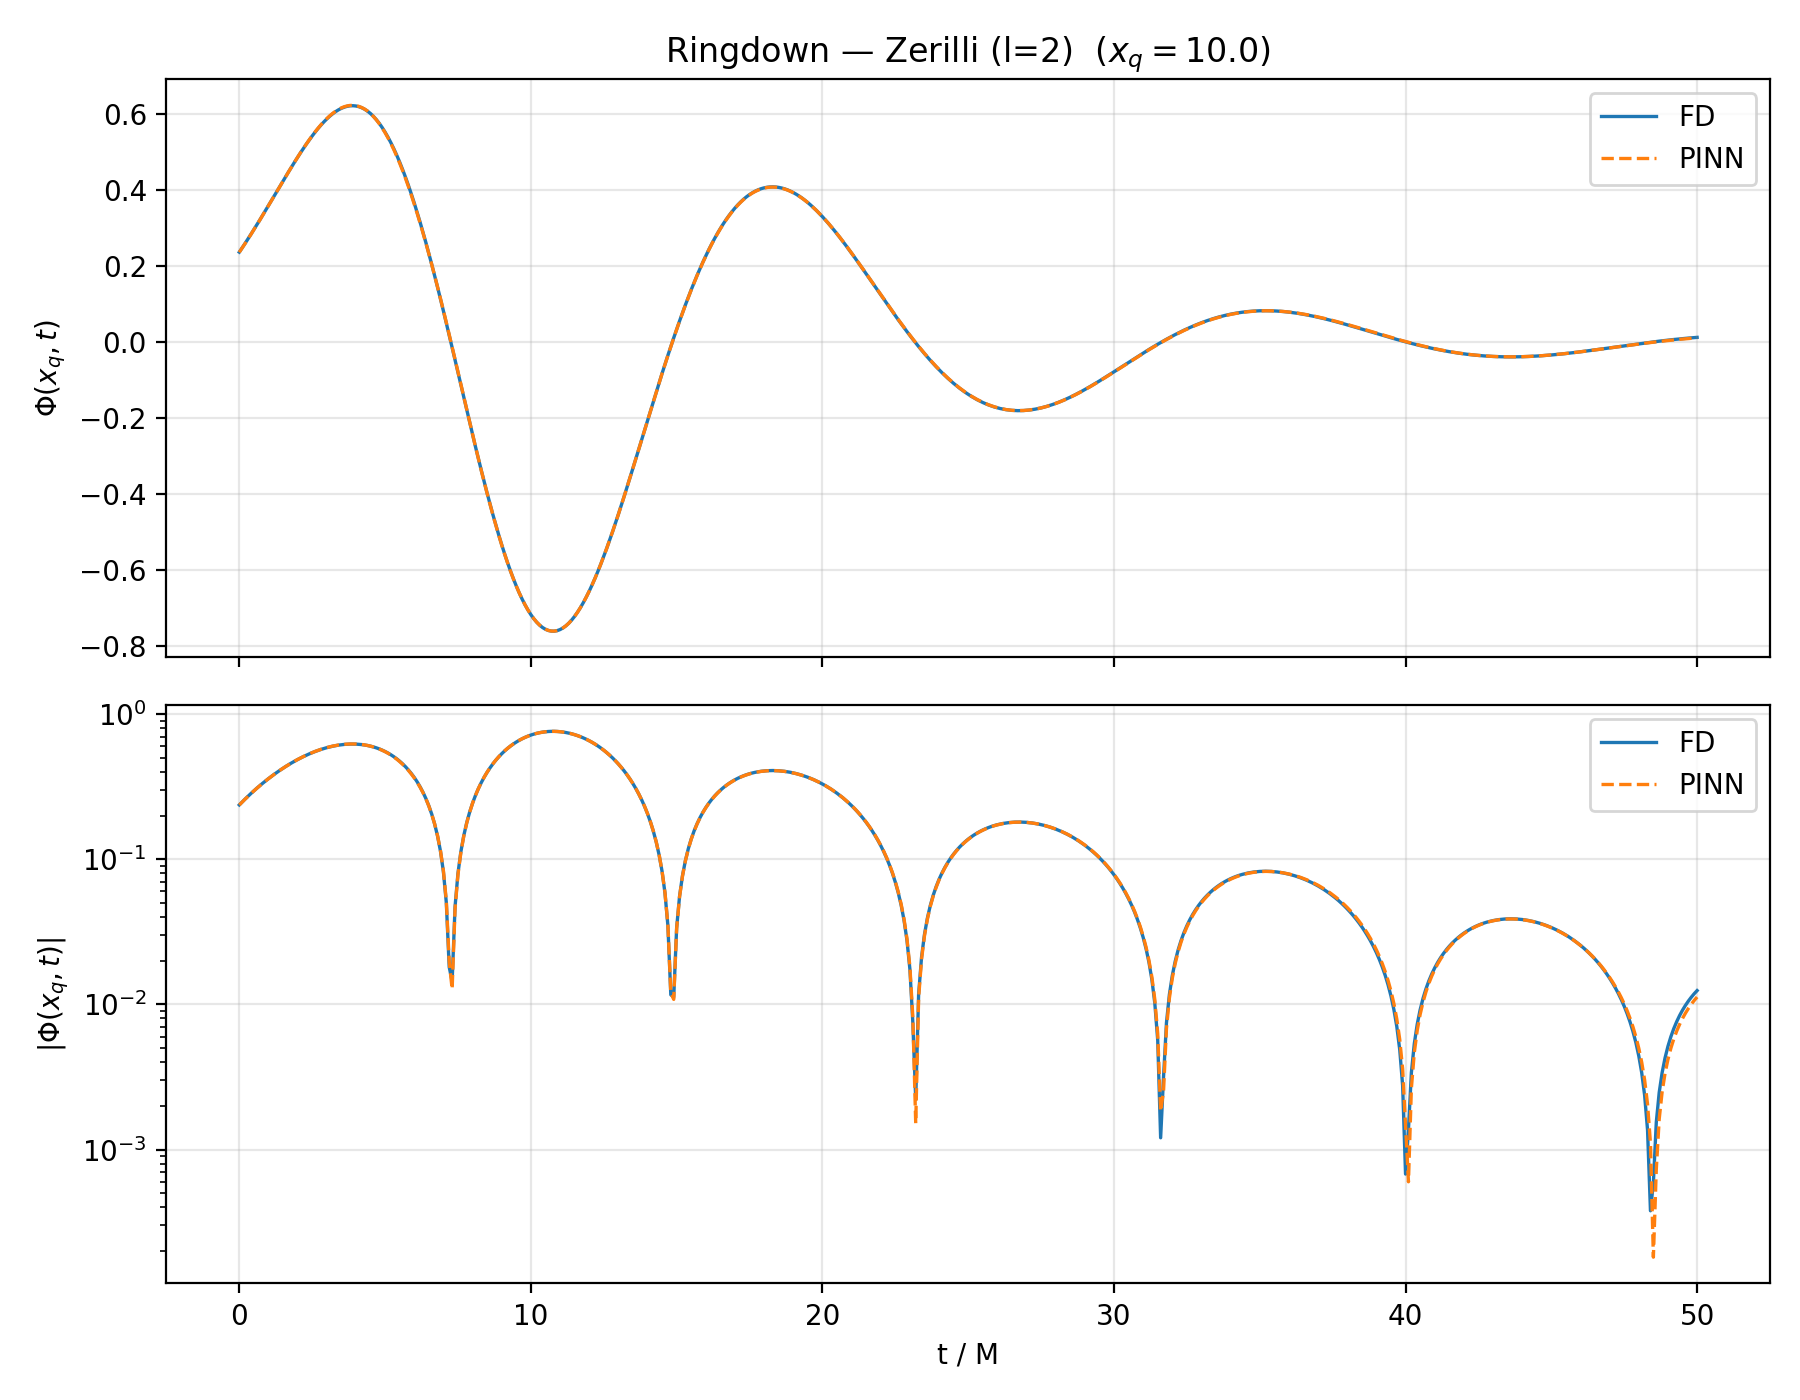
\includegraphics[width=\linewidth,height=0.70\textheight,keepaspectratio]{../outputs/pinn/zerilli_l2_greedy_f03_lbfgs30k/ringdown_overlay.png}
      \\[3pt]{\scriptsize Ringdown overlay at $\xq\!=\!10M$: PINN (solid) vs FD (dashed).
      Greedy $f\!=\!0.3$ + L-BFGS 30k.}
    \end{column}
  \end{columns}
\end{frame}

\begin{frame}{Forward PINN --- snapshots and pointwise error}
  \begin{columns}[T]
    \begin{column}{0.50\textwidth}
      \centering
      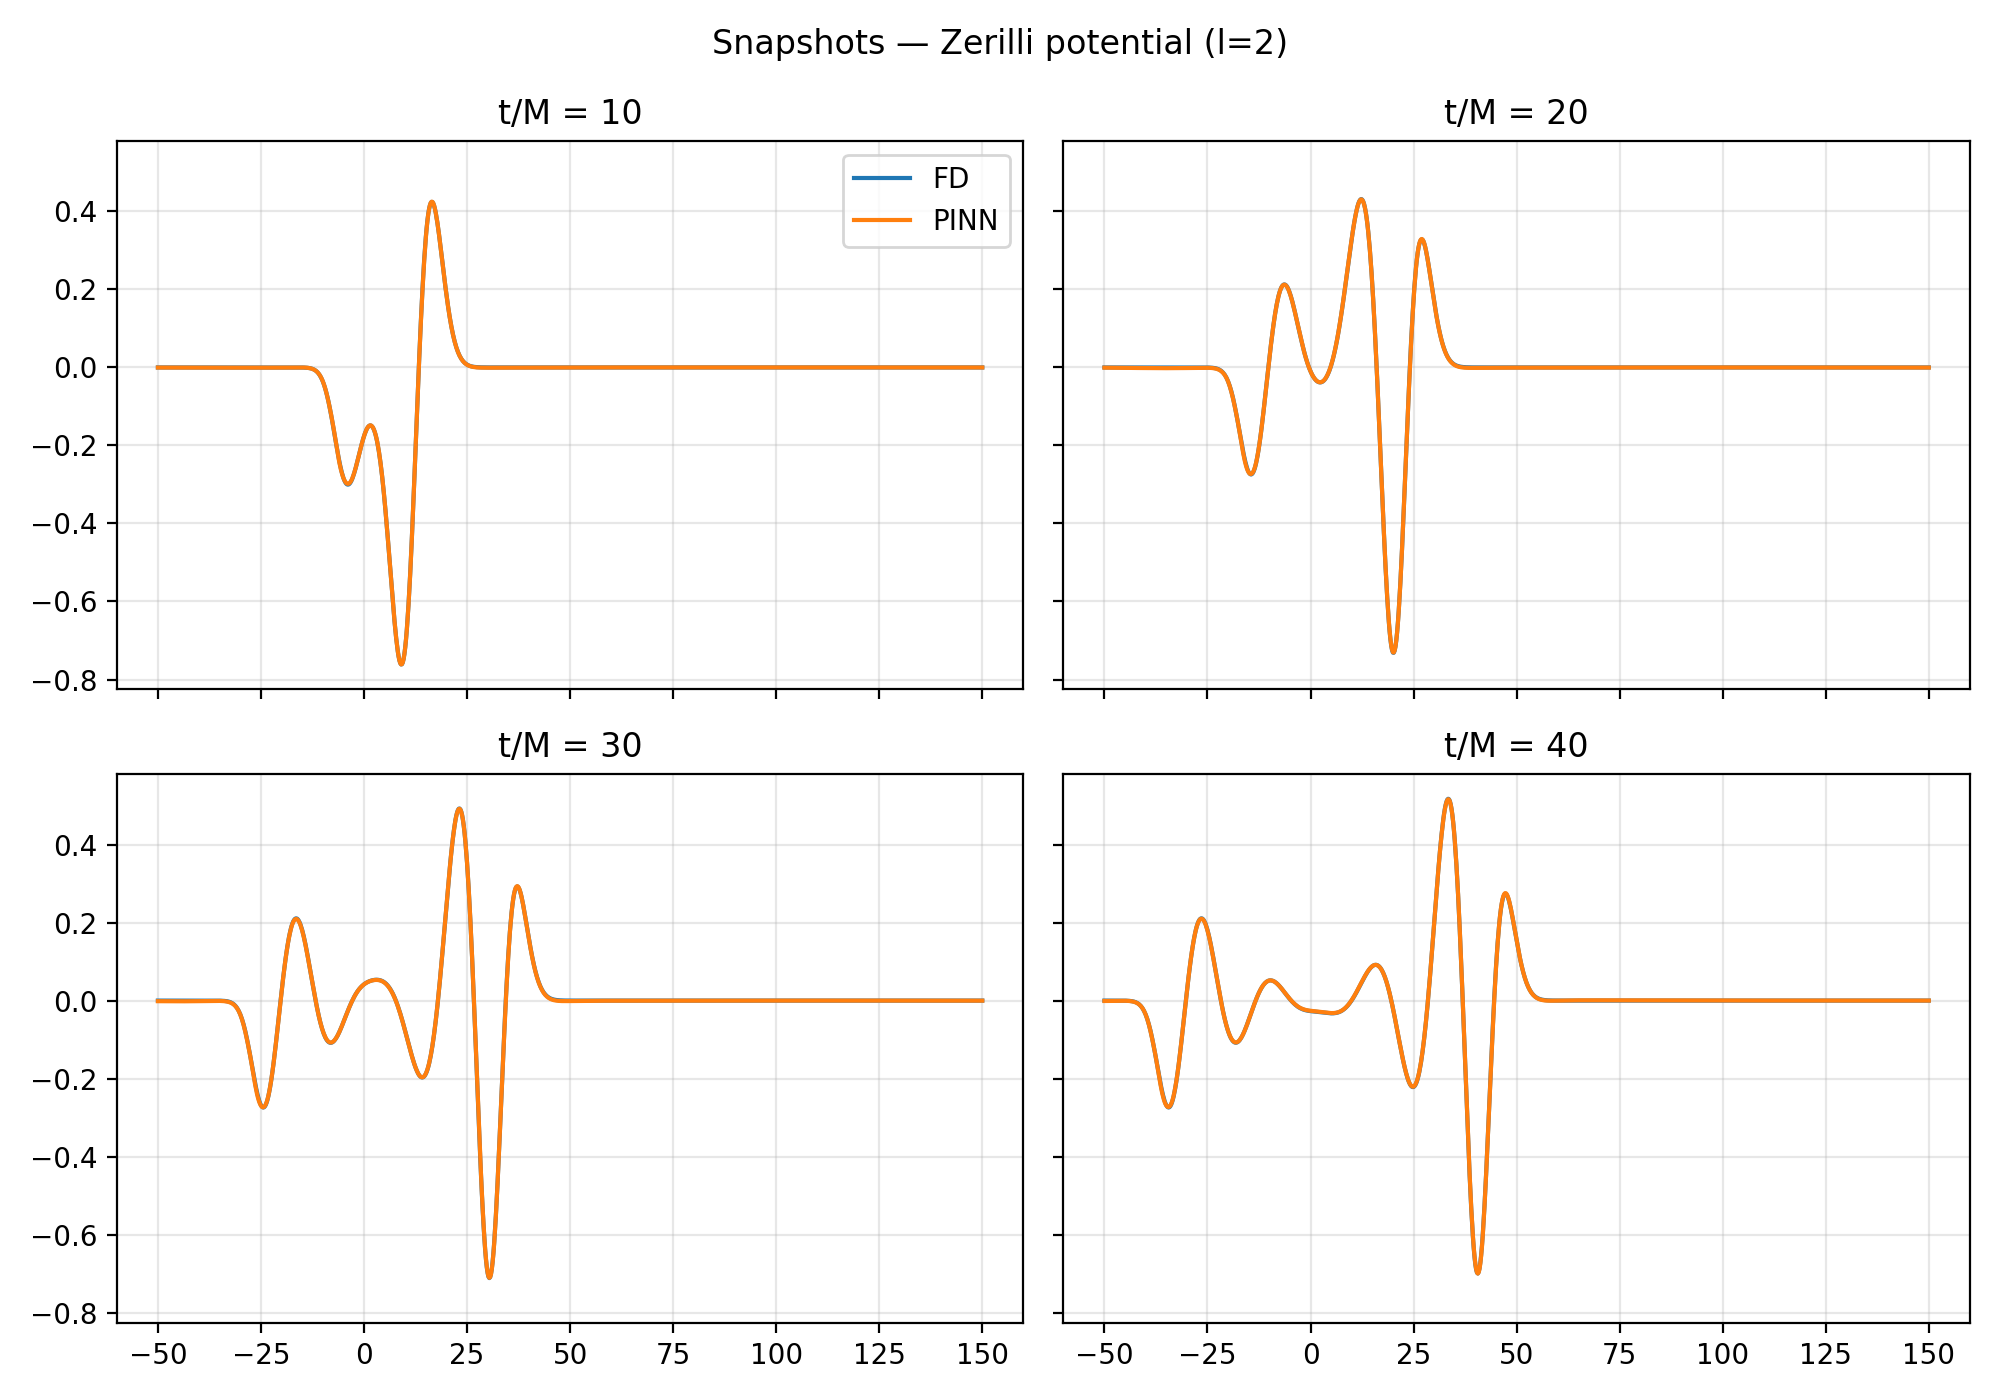
\includegraphics[width=\textwidth,height=0.72\textheight,keepaspectratio]{../outputs/pinn/zerilli_l2_greedy_f03_lbfgs30k/snapshots.png}
      \\[2pt]{\scriptsize $\Phi_{\pinn{}}$ (solid) vs $\Phi_{\fd{}}$ (dashed) at
      $t/M\!\in\!\{10,20,30,40\}$.}
    \end{column}
    \begin{column}{0.48\textwidth}
      \centering
      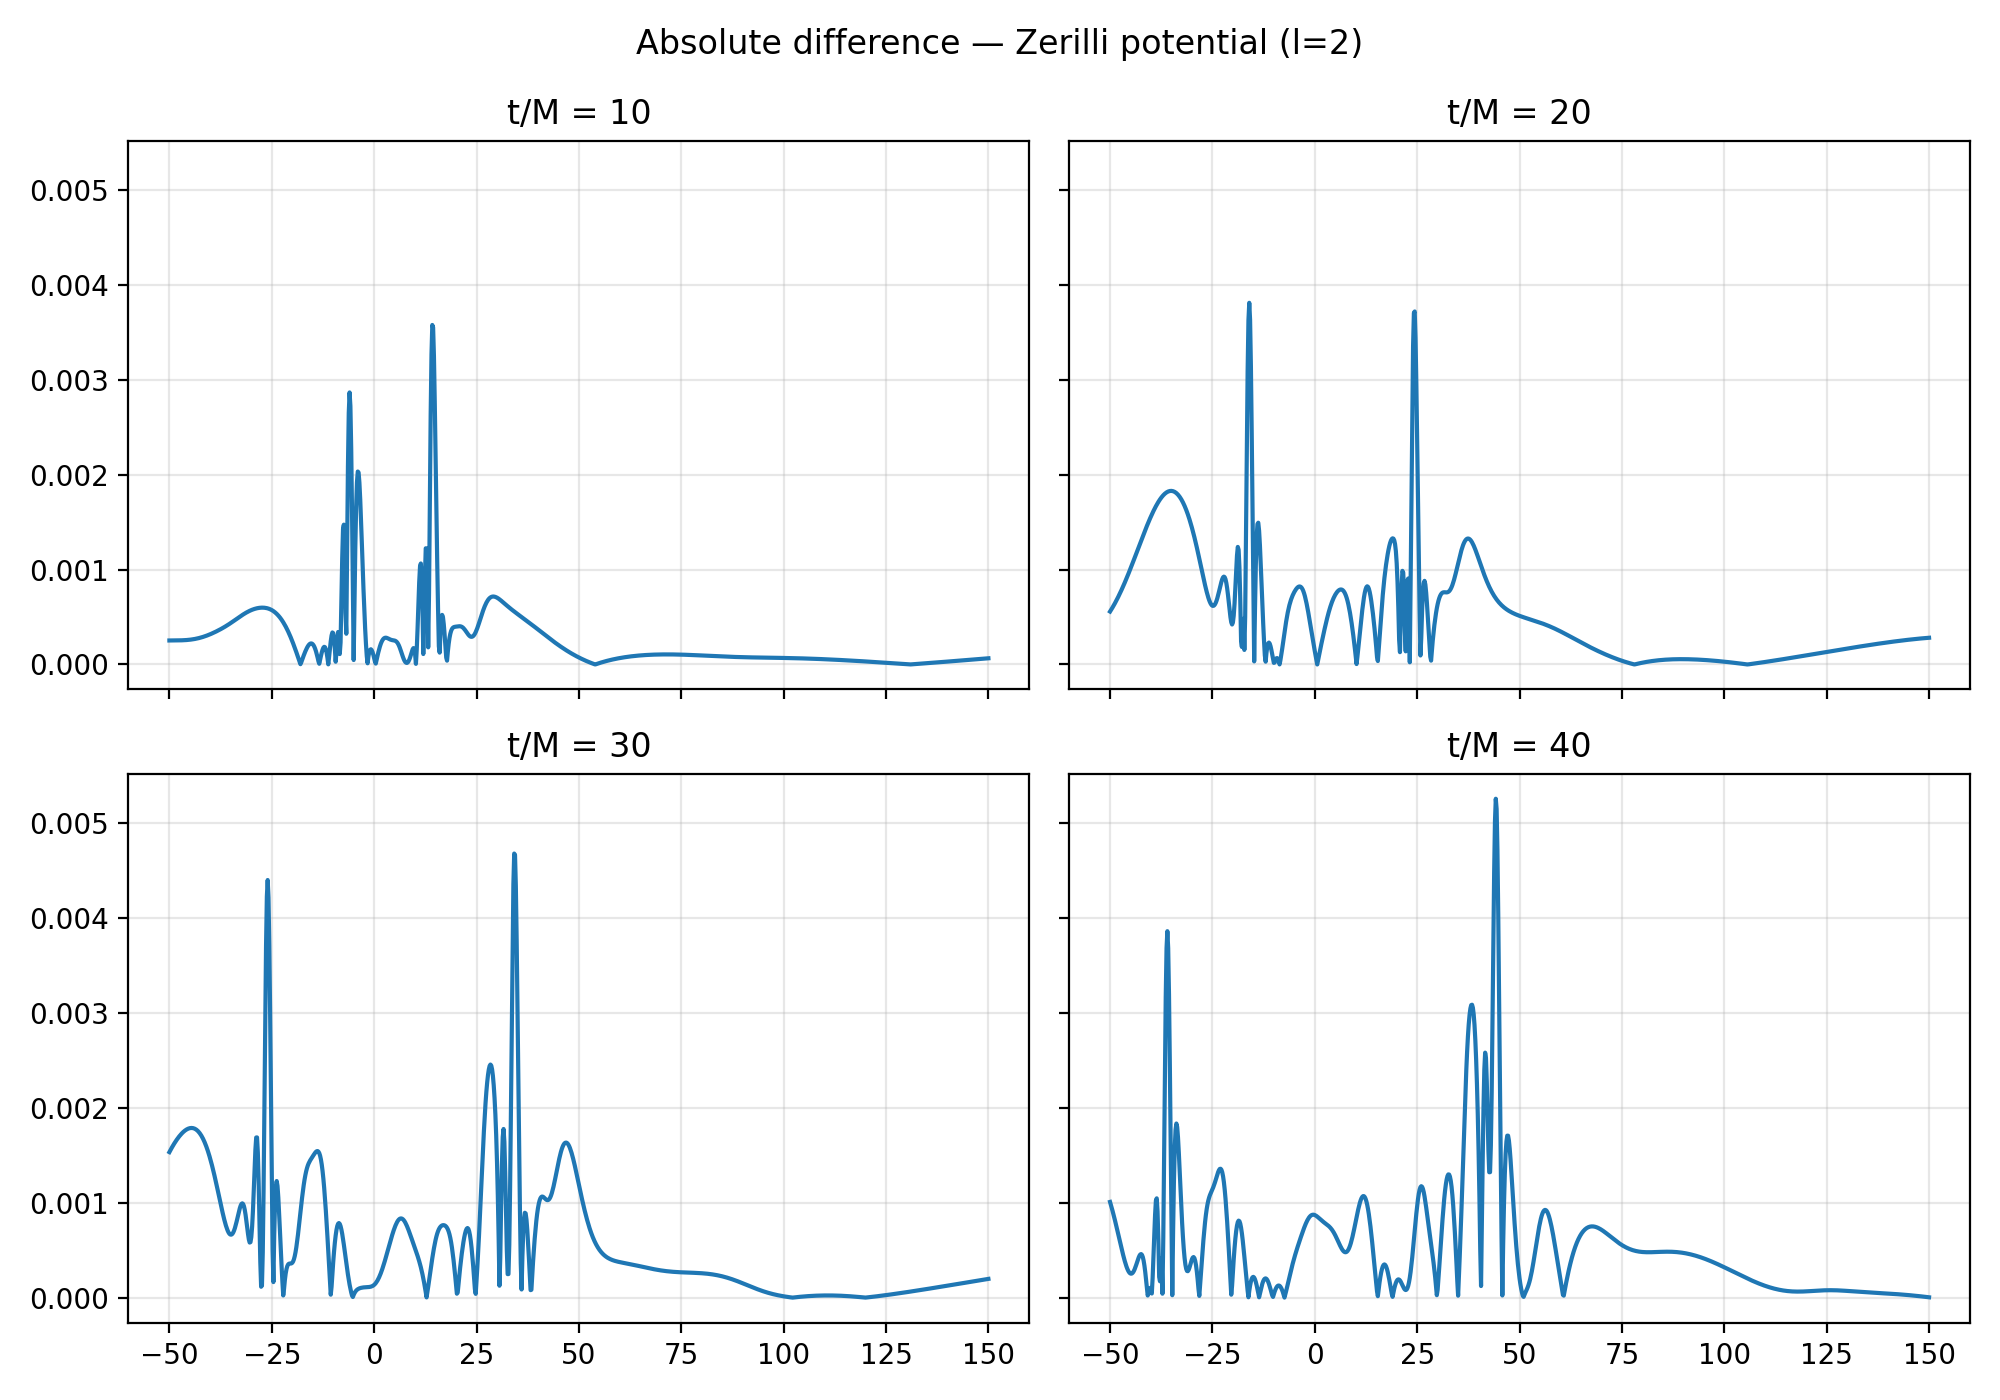
\includegraphics[width=\textwidth,height=0.72\textheight,keepaspectratio]{../outputs/pinn/zerilli_l2_greedy_f03_lbfgs30k/abs_diff_snapshots.png}
      \\[2pt]{\scriptsize Pointwise $|\Phi_{\pinn{}}-\Phi_{\fd{}}|$: residual
      $\lesssim\!5\!\times\!10^{-3}$ near the barrier, $\lesssim\!10^{-3}$ far away.}
    \end{column}
  \end{columns}
\end{frame}

\begin{frame}{Forward PINN --- best result: field $+$ QNM}
  \textbf{Field accuracy.} Gridwise RMSD vs FD $= 8.17\times10^{-4}$
  (relative $L^{2}\approx0.58\%$).
  \medskip
  \begin{center}\footnotesize
    \begin{tabular}{@{}lcccc@{}}
      \toprule
      \textbf{Method} & $\boldsymbol{\omega}$ & $\boldsymbol{\omega}$ \textbf{err} & $\boldsymbol{\tau}$ & $\boldsymbol{\tau}$ \textbf{err} \\
      \midrule
      Truth (Leaver)         & 0.3737  & ---     & 11.241 & ---     \\
      \midrule
      M1 (FFT + envelope)    & 0.3712  & 0.68\%  & 10.92  & 2.83\%  \\
      M2 (single-mode NLS)   & 0.3794  & 1.54\%  & 11.46  & \textbf{1.99\%}  \\
      M3 (ESPRIT)            & 0.4829  & 29.2\%  & 7.84   & 30.3\%  \\
      \rowcolor{green!10}
      M4 (two-mode plateau)  & 0.37359 & \textbf{0.029\%} & 10.94  & 2.65\%  \\
      M5 (2-D plateau)       & 0.37284 & 0.23\%  & 10.80  & 3.91\%  \\
      \bottomrule
    \end{tabular}
  \end{center}
  \medskip
  \begin{itemize}\small
    \item \textbf{Best $\omega$: M4 at 0.029\%} --- plateau + two-mode template
          removes overtone bias \emph{and} window arbitrariness.
    \item \textbf{Best $\tau$: M2 wide-window at 1.99\%.}
    \item M3 fails here (Hankel ill-conditioned at $\sim\!10^{-24}$ late amplitude) ---
          flagged automatically; the five-method spread is the cross-check.
  \end{itemize}
\end{frame}

\begin{frame}{Forward PINN --- greedy vs uniform error map}
  \begin{columns}[T]
    \begin{column}{0.50\textwidth}
      \centering
      
\includegraphics[width=\textwidth,height=0.72\textheight,keepaspectratio]{../../project32_qnm_pinn/outputs/pinn/zerilli_l2_paper/error_heatmap.png}
      \\[2pt]{\scriptsize Uniform baseline (Patel \emph{et al.}\ 2024 reproduction):
      residual along the outgoing wavefronts.}
    \end{column}
    \begin{column}{0.48\textwidth}
      \centering
      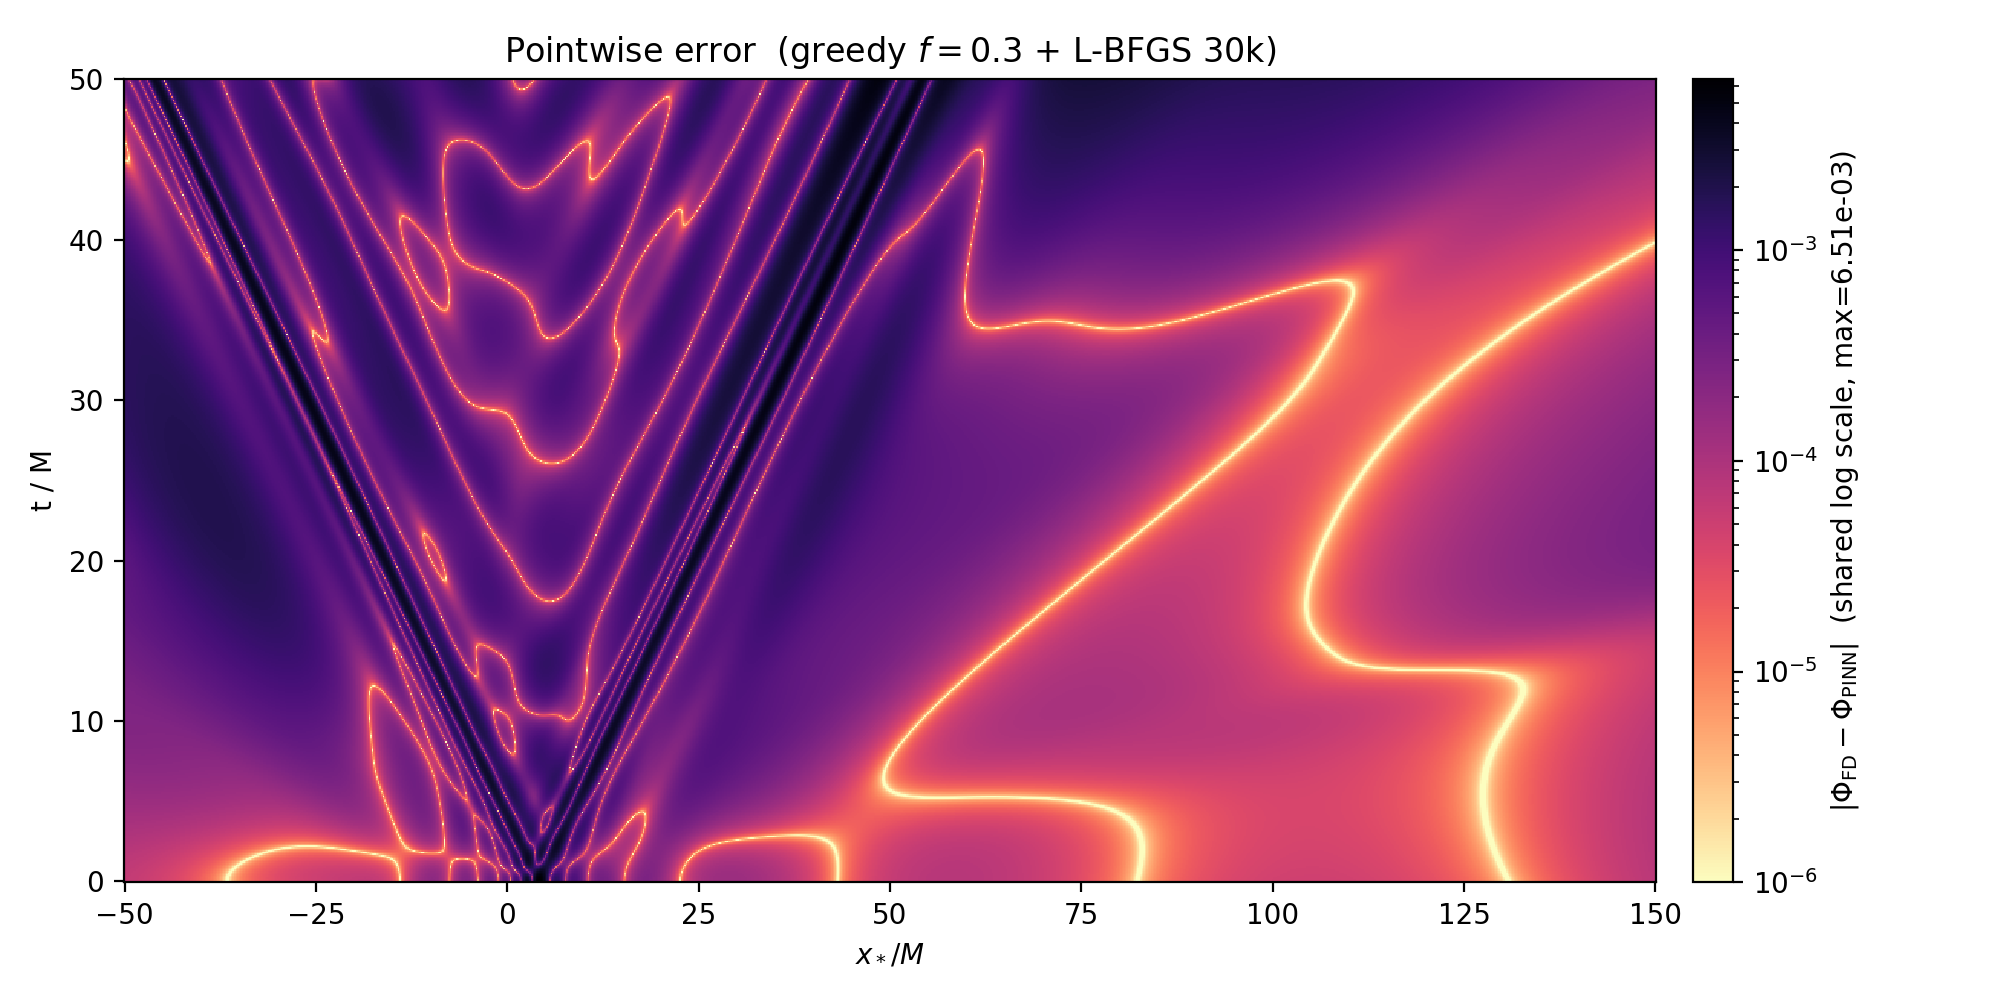
\includegraphics[width=\textwidth,height=0.72\textheight,keepaspectratio]{../outputs/pinn/zerilli_l2_greedy_f03_lbfgs30k/error_heatmap_compare.png}
      \\[2pt]{\scriptsize Greedy $f\!=\!0.3$ + L-BFGS 30k (same colour scale):
      wavefront residual visibly reduced (overall RMSD $-55\%$ vs uniform).}
    \end{column}
  \end{columns}
  \medskip
  \centering\small
  \fbox{\parbox{0.92\textwidth}{\centering
    Patel \emph{et al.}\ 2024: field error $28\%$, $\omega$ error $0.29\%$.\;
    \textbf{Our forward PINN: field $0.58\%$ ($\sim\!50\times$ tighter), $\omega$ $0.03\%$ (M4).}}}
\end{frame}


% ══════════════════════════════════════════════════════════════════
\section{5. Hybrid FNO Methodology}
% ══════════════════════════════════════════════════════════════════

\begin{frame}{Primer --- what is a Fourier Neural Operator?}
  A \pinn{} learns \emph{one} solution function $\Phi(x,t)$ and must be retrained for
  every new problem. A \textbf{neural operator} instead learns the \emph{solution map}
  itself --- a mapping between whole functions:
  \[
    \mathcal{G}_\theta:\; a(x)\;\longmapsto\;u(x),
  \]
  e.g.\ (initial data\,/\,coefficients) $\mapsto$ (solution field). Once trained it returns
  the solution for \emph{any} new input $a$ in a single forward pass --- no re-solving.
  \medskip
  \begin{block}{\footnotesize Architecture: lift $\to$ Fourier layers $\to$ project}
    \footnotesize
    \[
      a(x)\;\xrightarrow{\;P\;}\;v_0\;\xrightarrow{\ \text{Fourier}\ }\;v_1\to\cdots\to v_T
      \;\xrightarrow{\;Q\;}\;u(x)
    \]
    \begin{itemize}
      \item \textbf{Lift} $P$: pointwise ($1{\times}1$) MLP raises the few physical
            channels to a wide hidden width $d_v$.
      \item \textbf{$T$ Fourier layers} (here $L\!=\!4$): the global mixing --- next slide.
      \item \textbf{Project} $Q$: pointwise MLP maps the hidden width back to the output field.
    \end{itemize}
  \end{block}
  \medskip
  \footnotesize \textbf{Key property:} the learnable weights live in \emph{Fourier space},
  not on grid nodes $\Rightarrow$ the operator is (approximately)
  \textbf{discretisation-invariant} --- train on one grid, evaluate on a finer one.
\end{frame}

\begin{frame}{Primer --- inside a Fourier layer (the spectral convolution)}
  Each layer updates the hidden function with a \emph{local} path plus a \emph{global} path:
  \[
    v_{t+1}(x)=\sigma\!\Big(\underbrace{W\,v_t(x)}_{\text{local }1\times1\text{ conv}}
      \;+\;\underbrace{\big(\mathcal{K}v_t\big)(x)}_{\text{global spectral term}}\Big).
  \]
  The global term is a convolution, evaluated cheaply in frequency space (convolution
  theorem): FFT $\to$ keep the lowest $k_{\max}$ modes $\to$ multiply each by a learned
  complex weight $\to$ inverse FFT,
  \[
    \big(\mathcal{K}v_t\big)(x)=\mathcal{F}^{-1}\!\big(R_\theta\cdot\mathcal{F}(v_t)\big)(x),
    \qquad R_\theta\in\mathbb{C}^{\,k_{\max}\times d_v\times d_v}.
  \]
  \begin{itemize}\small
    \item \textbf{Global receptive field in one layer} --- every point couples to every
          other, matching the globally-coupled nature of PDE solution operators.
    \item \textbf{Mode truncation} (modes $>k_{\max}$ dropped): a low-frequency / smoothness
          prior, and cheap --- $\mathcal{O}(N\log N)$ via the FFT, not $\mathcal{O}(N^2)$.
    \item \textbf{Resolution invariance:} $R_\theta$ is indexed by mode number, not grid
          index --- refine the grid and the \emph{same} weights still apply.
    \item The local $W$ path restores the sharp / non-periodic features mode truncation discards.
  \end{itemize}
  \medskip
  \footnotesize \textbf{Next:} we do not learn the \emph{whole} wave operator with an
  \fno{} --- we use one only for the bounded \emph{residual} a cheap coarse solver misses.
\end{frame}

\begin{frame}{Hybrid FNO --- the idea}
  A \pinn{} (or an end-to-end neural operator) learns the \emph{entire}
  wave-propagation operator from scratch. \textbf{Alternative:} keep a cheap
  classical solver as the workhorse and ask the network \emph{only} for the part
  it cannot resolve.
  \medskip
  \begin{block}{\footnotesize Hybrid coarse-FD $+$ neural-residual surrogate}
    \footnotesize
    \begin{enumerate}
      \item Run \emph{one} inexpensive \textbf{coarse} ($k\!=\!4$) FD solve; upsample
            it to the fine grid $\Rightarrow$ the \emph{prior} $\Uop\Phi^{\mathrm{c}}$.
      \item A 2-D \fno{} predicts the \textbf{discretisation residual} the coarse solve misses.
      \item The target is built by \textbf{label-free Richardson extrapolation} of two
            coarse solves --- \emph{no fine-grid ground truth is ever used in training}.
      \item A parameter-free \textbf{gradient gate} confines the correction to the
            under-resolved wavefronts.
    \end{enumerate}
  \end{block}
  \medskip
  \footnotesize Cost of the classical part at inference: $k^{-3}=1/64$ of a fine FD solve.
\end{frame}

\begin{frame}{Hybrid FNO --- where the coarse prior fails}
  \centering
  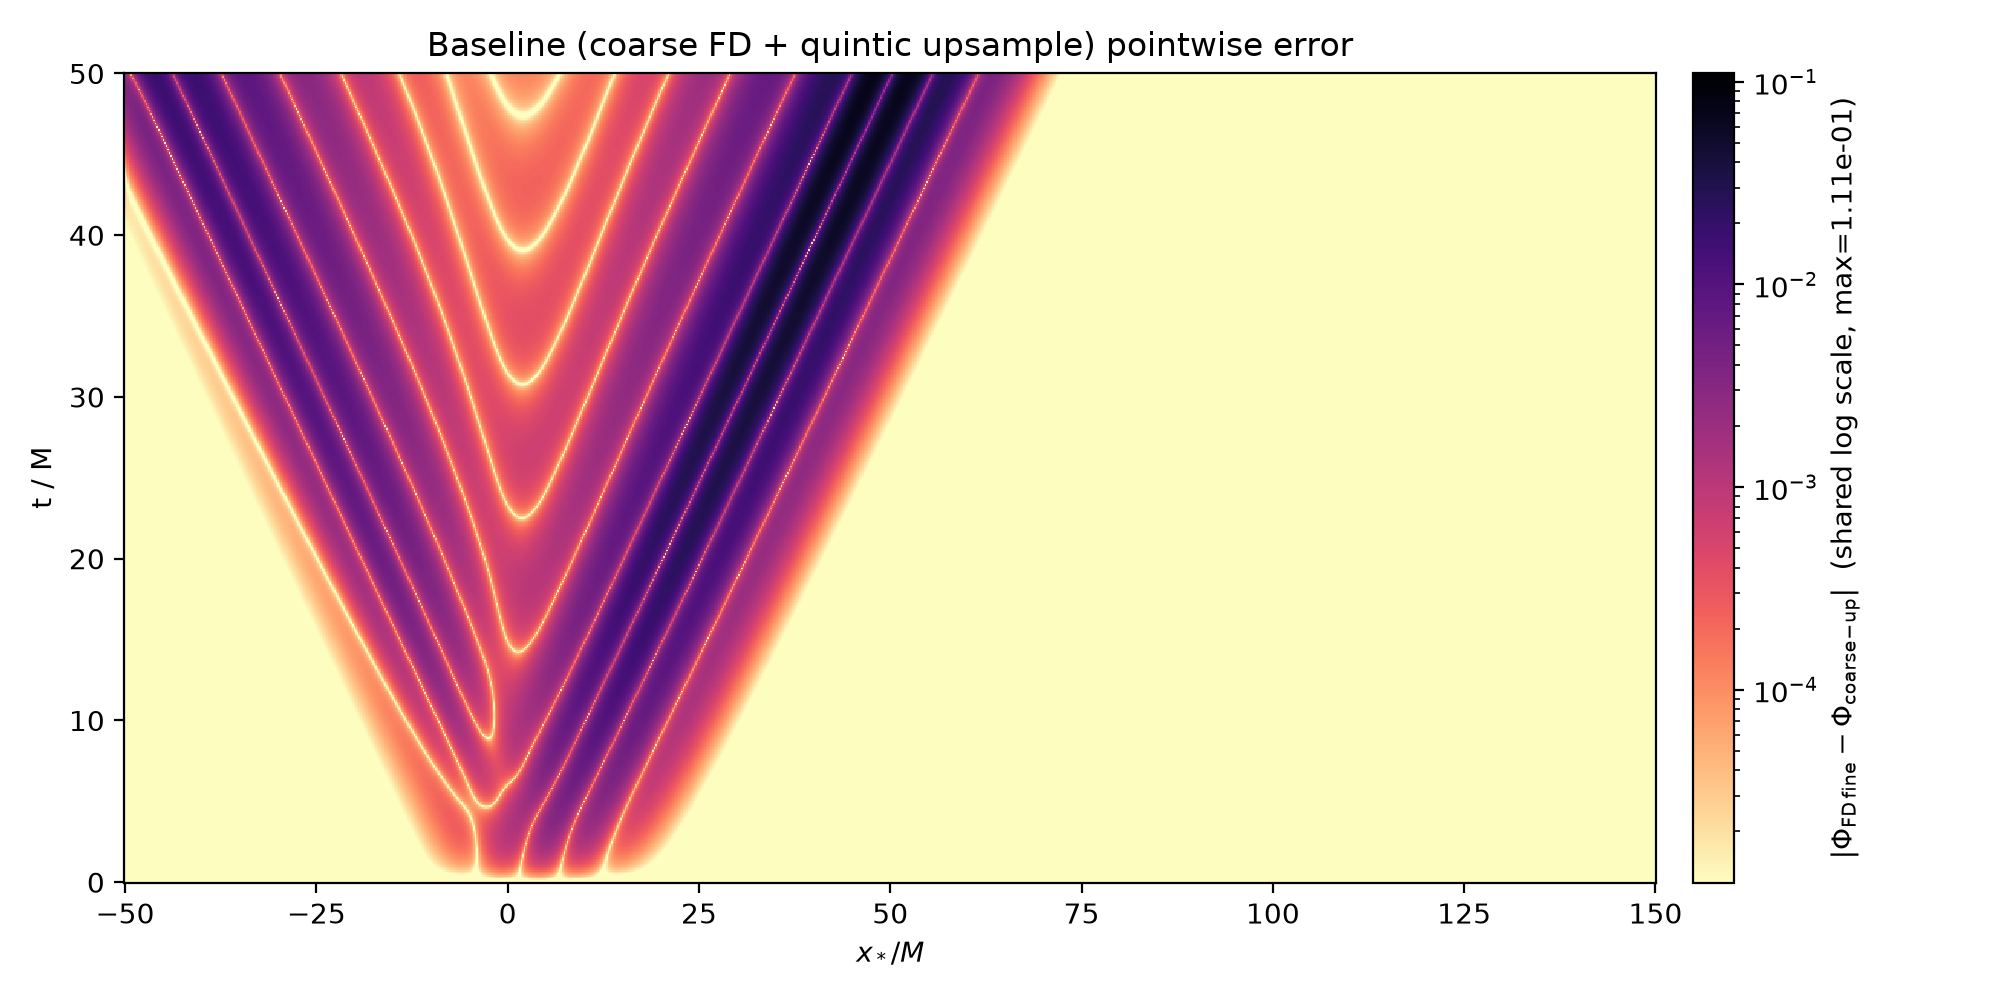
\includegraphics[width=0.82\textwidth,height=0.74\textheight,keepaspectratio]{../outputs/hybrid/fno_sw_gate_s1em3/figs/hybrid_pointwise_error_baseline.png}
  \\[2pt]
  \begin{minipage}{0.92\textwidth}\centering\footnotesize
    Pointwise error of the cheap $k\!=\!4$ coarse prior against the fine-FD reference
    (same magma\_r log scale as every error map in this talk). The error is
    \textbf{concentrated on the outgoing wavefronts} and near-zero in the smooth interior
    and causal exterior --- a \emph{bounded, spatially-localised} target. This is exactly
    the structure the gated hybrid FNO is built to repair.
  \end{minipage}
\end{frame}

\begin{frame}{Hybrid FNO --- the pipeline}
  \vfill
  \begin{center}
    {\Large The full hybrid surrogate pipeline}
    \par\medskip
    \fbox{\textbf{See report, p.~XX \quad(Sec.~3.6, Fig.~4 --- hybrid surrogate pipeline).}}
    \par\bigskip
    {\footnotesize At a glance:\;
     coarse $k\!=\!4$ FD $\to$ quintic upsample (prior) $\to$ 2-D FNO residual
     $\to$ gradient gate $\to$ $+\,$prior $=\Phi^{\mathrm{hyb}}$.\\[2pt]
     Training target (label-free): Richardson extrapolation of the $k\!=\!4$ and $k\!=\!2$
     coarse solves.}
  \end{center}
  \vfill
\end{frame}

\begin{frame}{Hybrid FNO --- label-free Richardson target}
  The $k\!=\!4$ prior is deliberately weak: its default 2nd-order stencil leaves an
  $\mathcal{O}(\Delta x_{\mathrm c}^{2})$ dispersion error ($6.1\%$ relative $L^2$).
  Rather than buy a better stencil, we \textbf{cancel} the leading error with two
  coarse solves:
  \[
    \Phi^{\mathrm{R}}=\frac{4\,\Uop\Phi^{\mathrm{c}}_{2}-\Uop\Phi^{\mathrm{c}}}{3}
    =\Phi+\mathcal{O}(\Delta x_{\mathrm c}^{4}),
    \qquad
    \delta\Phi_{\mathrm{R}}=\Phi^{\mathrm{R}}-\Uop\Phi^{\mathrm{c}} .
  \]
  \begin{itemize}\small
    \item The network is trained to predict $\delta\Phi_{\mathrm{R}}$ ---
          its loss \textbf{never sees the fine FD field}. Self-supervised from coarse solves.
    \item At inference only the single $k\!=\!4$ solve is needed
          ($k^{-3}=1/64$ of fine-FD cost); the $k\!=\!2$ solve is a training artefact.
    \item Quintic upsample $\Uop$: $\mathcal{O}(\Delta x_{\mathrm c}^{6})$ interpolation
          error stays below the $\mathcal{O}(\Delta x_{\mathrm c}^{4})$ Richardson signal.
  \end{itemize}
  \medskip
  \footnotesize \textbf{Weak prior $+$ Richardson} is the opposite of a strong classical
  stencil: cheapest possible solver, network does correspondingly more --- the regime where
  the $k^{d+1}$ saving is largest and which scales to higher dimensions.
\end{frame}

\begin{frame}{Hybrid FNO --- the gradient gate (key innovation)}
  The network correction is modulated by a \textbf{parameter-free} gate before being
  added to the prior:
  \[
    \Phi^{\mathrm{hyb}}=\Uop\Phi^{\mathrm{c}}+g(x,t)\,\mathcal{H}_\theta(X),
    \qquad
    g=\frac{|\nabla\Uop\Phi^{\mathrm{c}}|}{|\nabla\Uop\Phi^{\mathrm{c}}|+s},
    \quad s=10^{-3}.
  \]
  \begin{itemize}\small
    \item $g\!\to\!1$ on the high-gradient \textbf{wavefronts}, where the coarse prior
          dephases and carries its dispersion error.
    \item $g\!\to\!0$ in the smooth interior and the causal exterior, where the prior is
          already machine-accurate.
    \item Adds \emph{no} trainable parameters; the scale $s$ is fixed \emph{label-free}
          from the prior gradient distribution (68th percentile), within $2\%$ of the
          field-RMSD optimum.
    \item \textbf{Hard guarantee:} wherever $g\!=\!0$ the hybrid \emph{is} the coarse
          prior --- the network cannot pollute the regions the solver already resolves.
  \end{itemize}
  \medskip
  \footnotesize The gate rests on a testable hypothesis --- \emph{the coarse-prior error
  is large exactly where the prior gradient is large} --- which the next slide verifies.
\end{frame}

\begin{frame}{The gate hypothesis, verified}
  \centering
  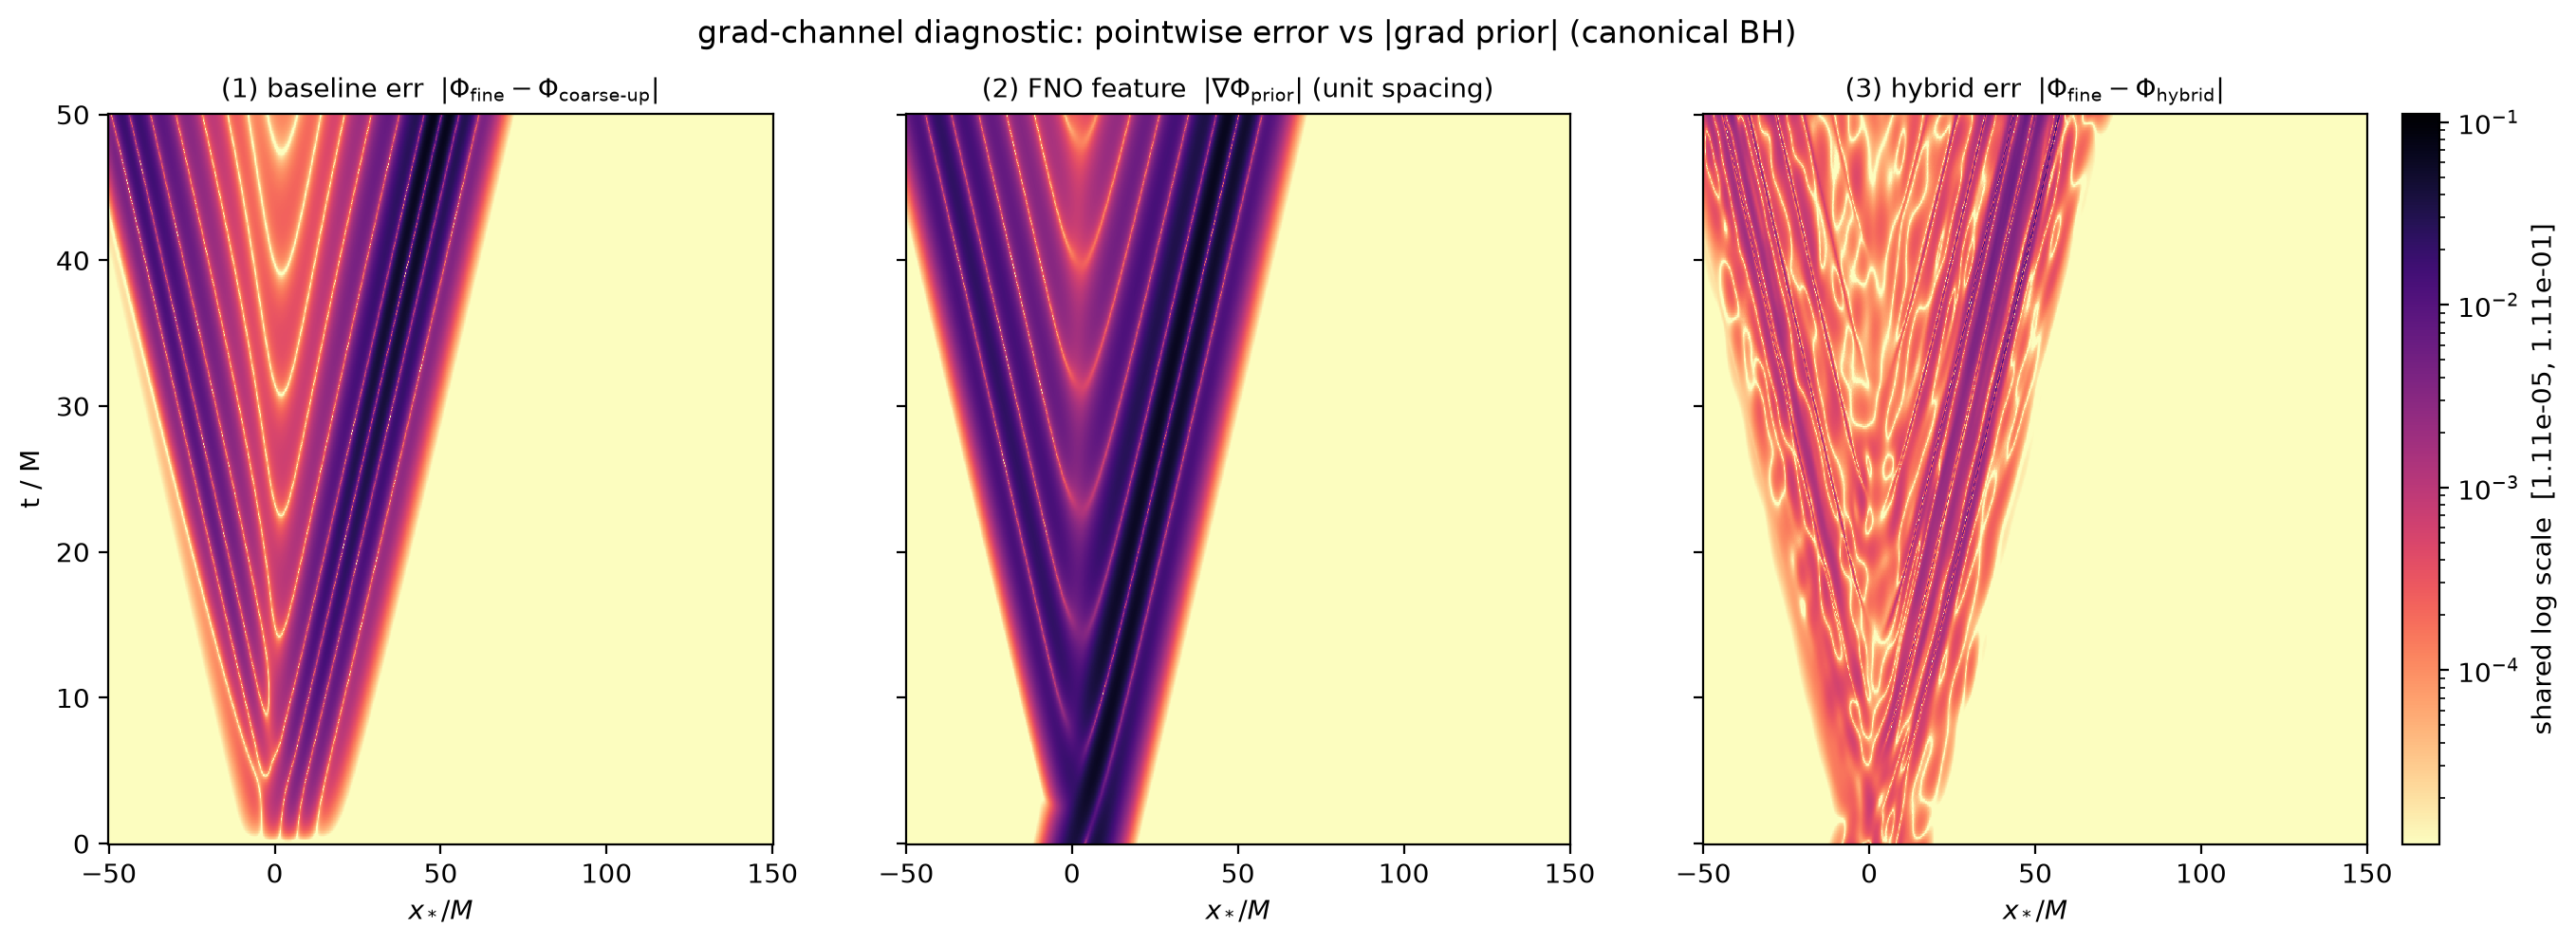
\includegraphics[width=0.96\textwidth,height=0.66\textheight,keepaspectratio]{../outputs/hybrid/fno_sw_gate_s1em3/figs/grad_vs_error.png}
  \\[2pt]
  \begin{minipage}{0.95\textwidth}\centering\footnotesize
    Grad-channel diagnostic on the canonical BH, all panels on the shared log scale:
    \textbf{(1)} coarse-prior error $|\Phi^{\mathrm{f}}-\Uop\Phi^{\mathrm{c}}|$,\;
    \textbf{(2)} the prior-gradient feature $|\nabla\Uop\Phi^{\mathrm{c}}|$ that defines the
    gate,\; \textbf{(3)} hybrid residual $|\Phi^{\mathrm{f}}-\Phi^{\mathrm{hyb}}|$.
    Panels (1) and (2) share the \emph{same} wavefront structure --- the prior fails exactly
    where its gradient is large (per-cell log--log Pearson $r=0.917$) --- so the gate routes
    the correction there; panel (3) shows it repaired.
  \end{minipage}
\end{frame}

\begin{frame}{Hybrid FNO --- network and cost}
  \begin{columns}[T]
    \begin{column}{0.56\textwidth}
      \textbf{Residual operator $\mathcal{H}_\theta$ (2-D FNO):}
      \begin{itemize}\small
        \item \textbf{5-channel input:} upsampled prior, $\Phi^{\mathrm{c}}(x,0)$,
              potential $V_\ell(x;M)$, mass $M$, coarse initial velocity $\Pi^{\mathrm{c}}_0$.
        \item lift $1{\times}1$ conv $5\!\to\!32$; \;$L\!=\!4$ Fourier layers;
              projection $32\!\to\!1$.
        \item $\sim\!1.13\times10^{6}$ parameters ($\sim\!70\times$ smaller than the
              end-to-end FNO).
        \item Adam, lr $10^{-3}$, label-free target, fine grid $1001\times501$.
      \end{itemize}
    \end{column}
    \begin{column}{0.44\textwidth}
      \begin{block}{\footnotesize Why hybrid, not end-to-end?}
        \footnotesize
        The network sits \emph{in series} with a classical solver that already gives a
        good guess, so it \textbf{inherits the stability and discretisation-invariance}
        of the FD scheme as a hard prior, and only repairs a bounded, localised residual.
      \end{block}
      \begin{block}{\footnotesize Deployment cost}
        \footnotesize
        One $k\!=\!4$ solve ($1/64$ fine-FD) $+$ one FNO forward pass, for \emph{any}
        $(M,x_0,\sigma)$ in the family --- \emph{no retraining}.
      \end{block}
    \end{column}
  \end{columns}
\end{frame}


% ══════════════════════════════════════════════════════════════════
\section{6. Hybrid FNO Results}
% ══════════════════════════════════════════════════════════════════

\begin{frame}{Hybrid FNO --- field accuracy}
  \begin{columns}[T]
    \begin{column}{0.56\textwidth}
      \centering
      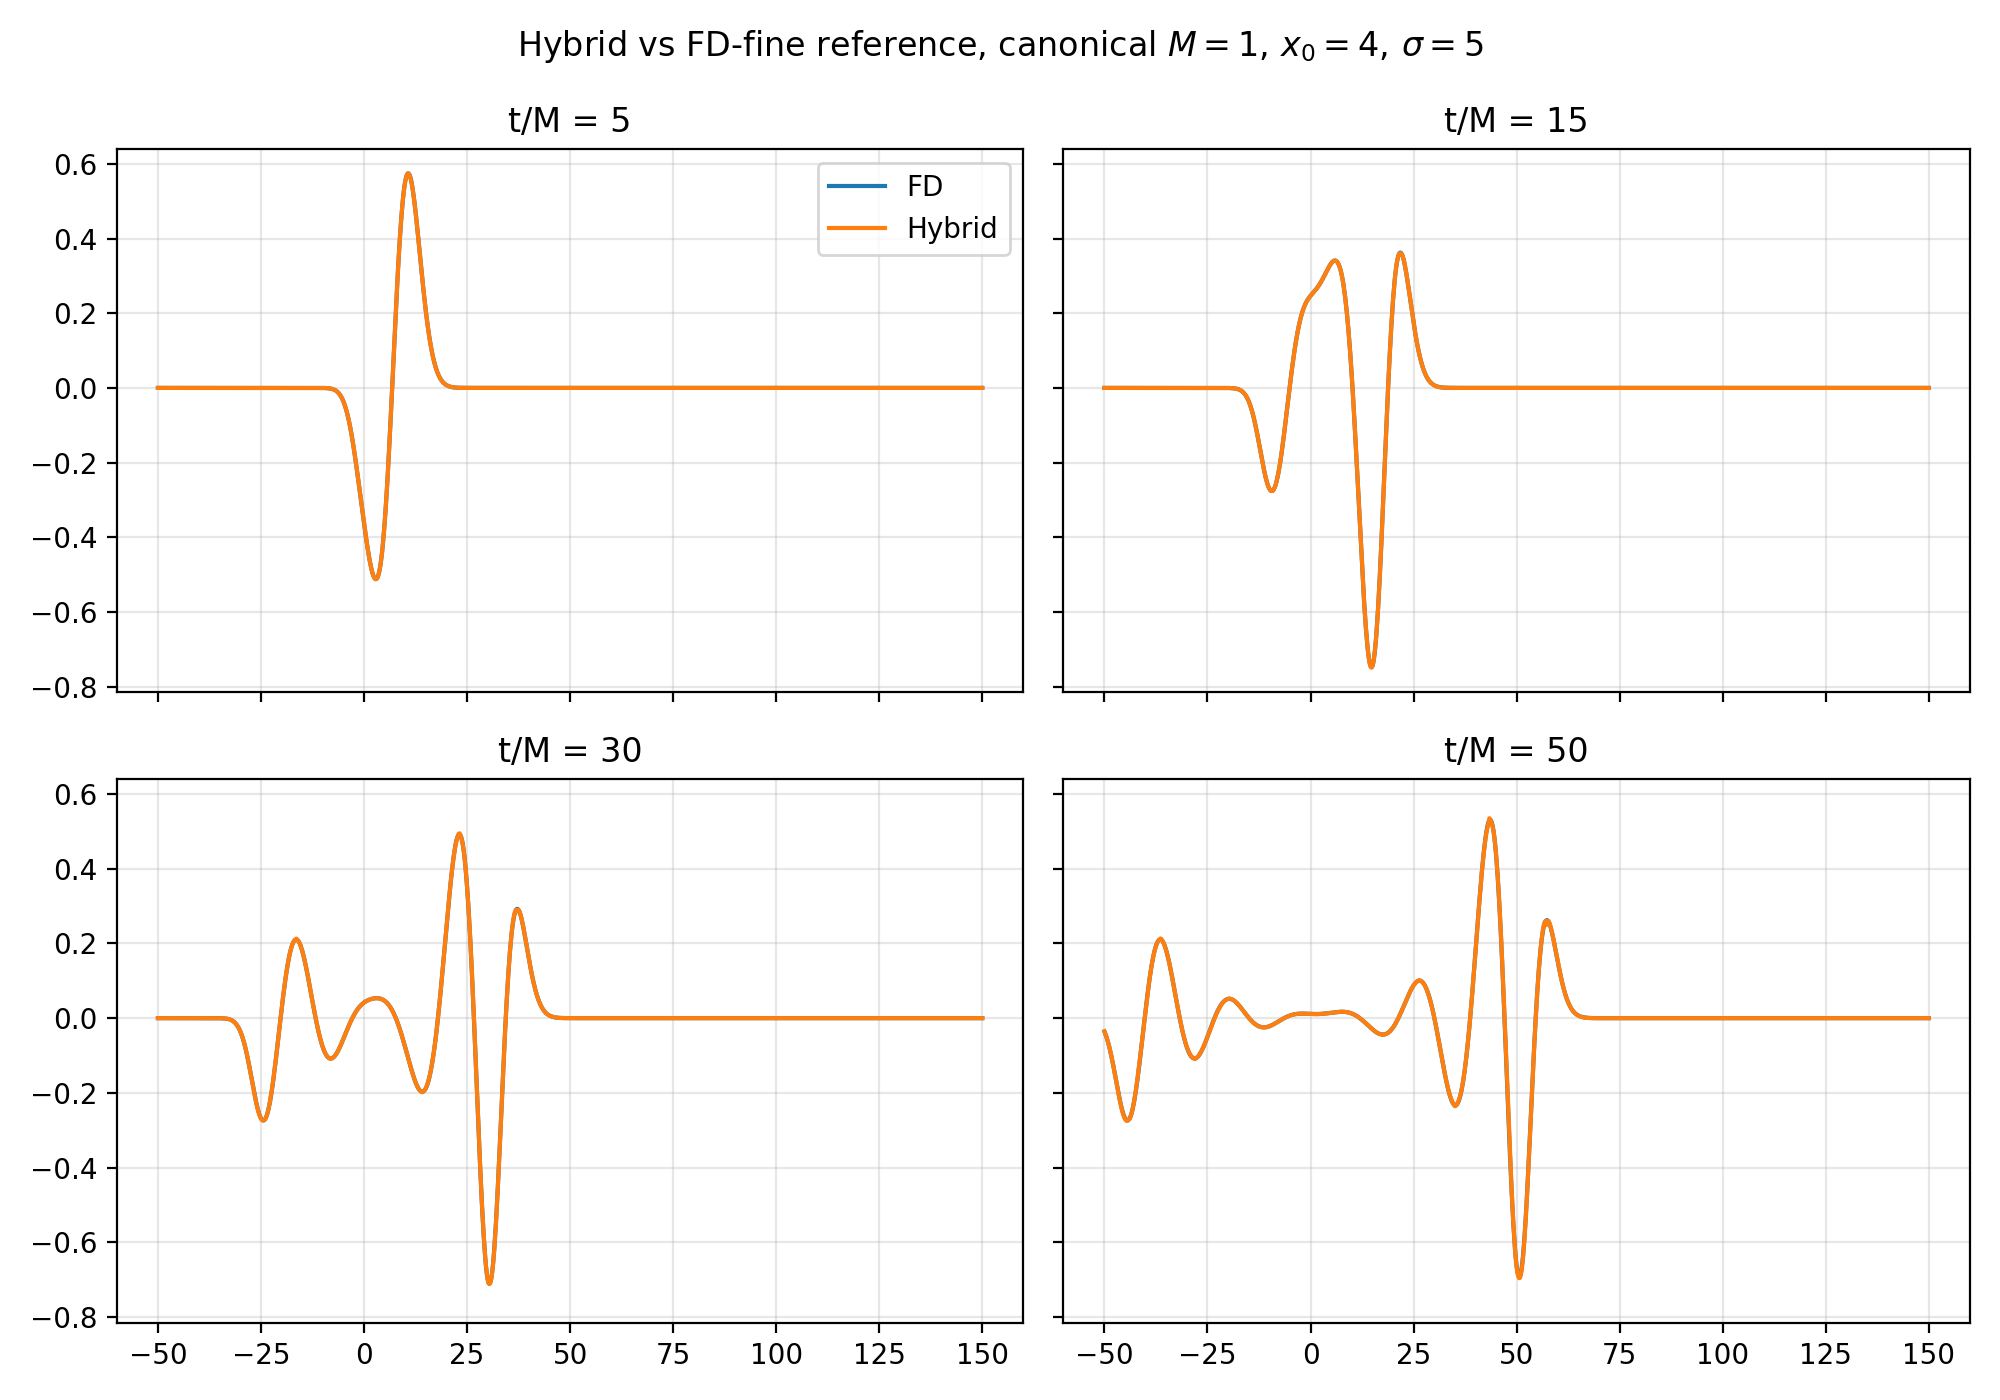
\includegraphics[width=\textwidth,height=0.74\textheight,keepaspectratio]{../outputs/hybrid/fno_sw_gate_s1em3/figs/hybrid_snapshots.png}
      \\{\scriptsize Hybrid (orange) vs fine FD (blue) at $t/M\!\in\!\{5,15,30,50\}$ ---
      indistinguishable on this scale.}
    \end{column}
    \begin{column}{0.44\textwidth}
      \textbf{Field error (relative $L^2$):}
      \begin{center}\footnotesize
        \begin{tabular}{@{}lcc@{}}
          \toprule
           & coarse prior & \textbf{hybrid} \\
          \midrule
          canonical \bh{} & $4.93\%$ & \textbf{$0.49\%$} \\
          $100$-\bh{} median & $6.11\%$ & \textbf{$0.67\%$} \\
          \bottomrule
        \end{tabular}
      \end{center}
      \medskip
      \begin{itemize}\small
        \item $\mathbf{10.1\times}$ field gain on the canonical \bh{},
              $\mathbf{9.1\times}$ across the population ($79\times$ in MSE).
        \item Consistent across the whole training family --- not a single-draw artefact.
        \item The residual lives \emph{only} on the outgoing wavefronts.
      \end{itemize}
    \end{column}
  \end{columns}
\end{frame}

\begin{frame}{Hybrid FNO --- the gate works}
  \begin{columns}[T]
    \begin{column}{0.56\textwidth}
      \centering
      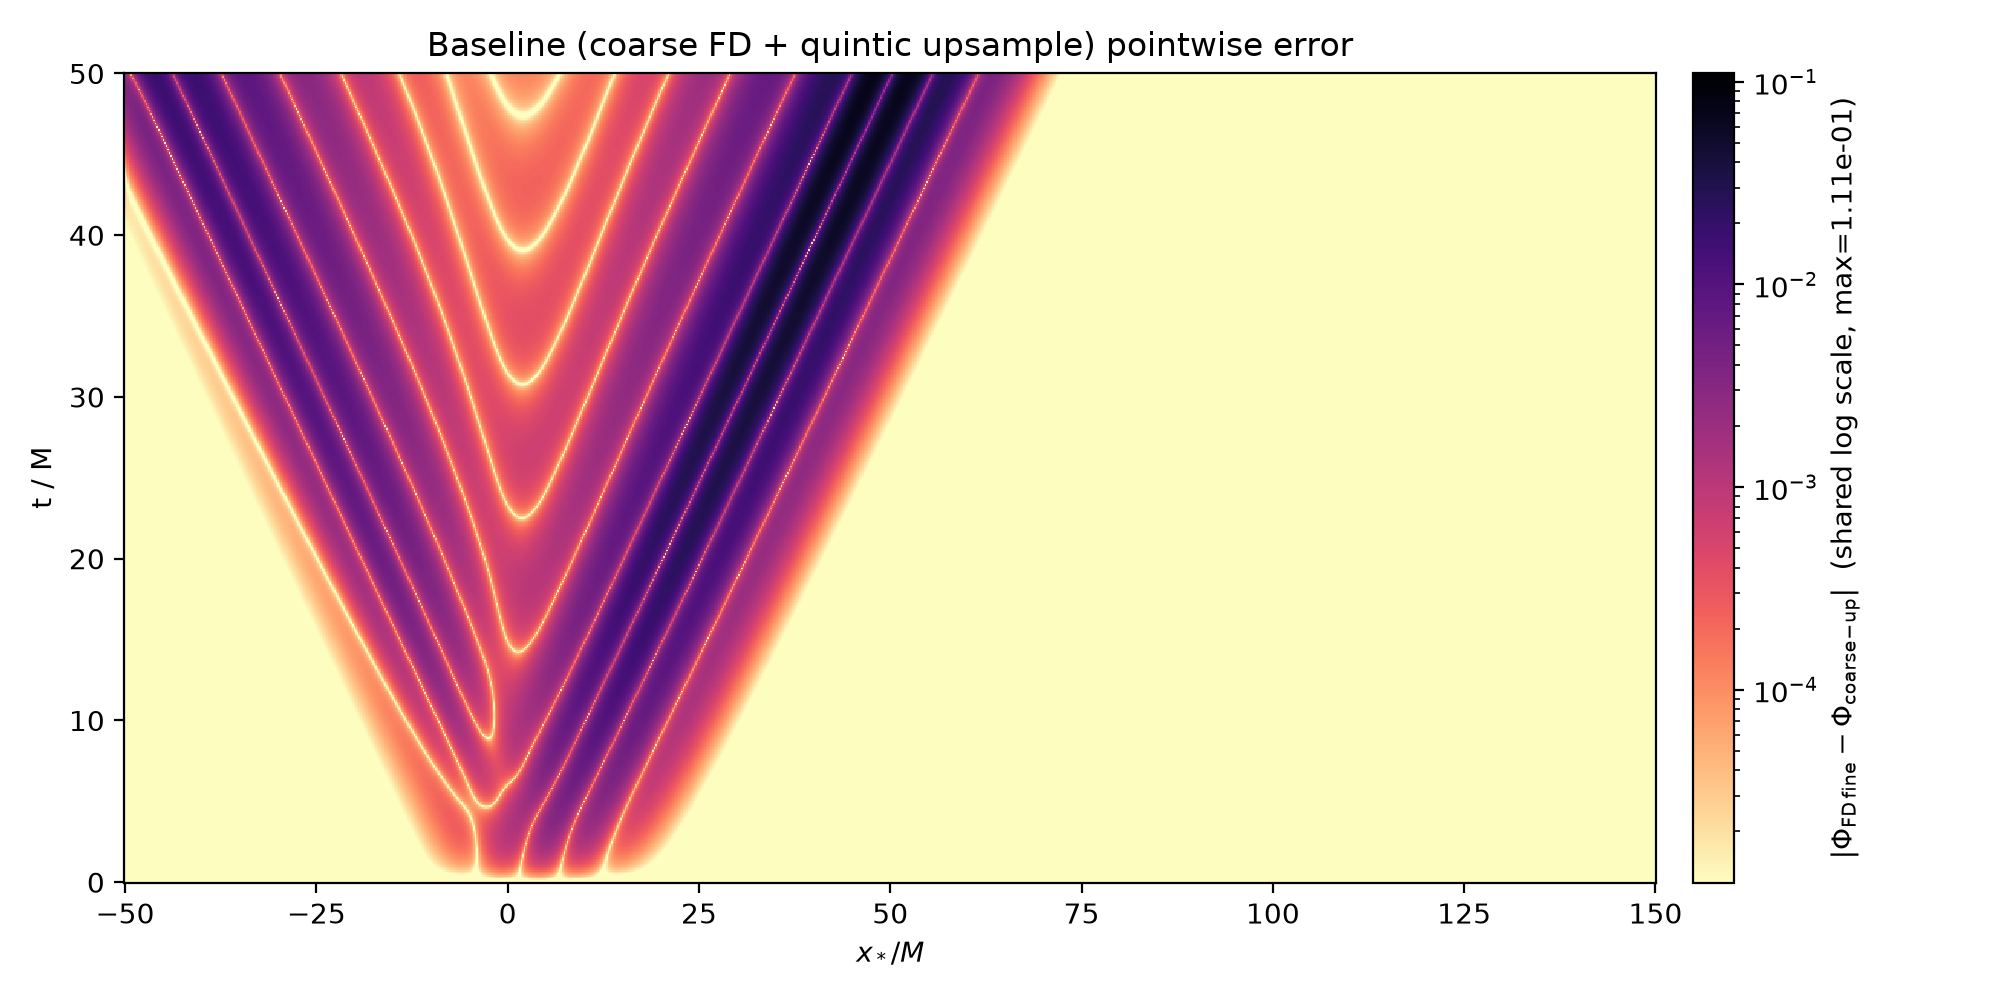
\includegraphics[width=\textwidth,height=0.46\textheight,keepaspectratio]{../outputs/hybrid/fno_sw_gate_s1em3/figs/hybrid_pointwise_error_baseline.png}
      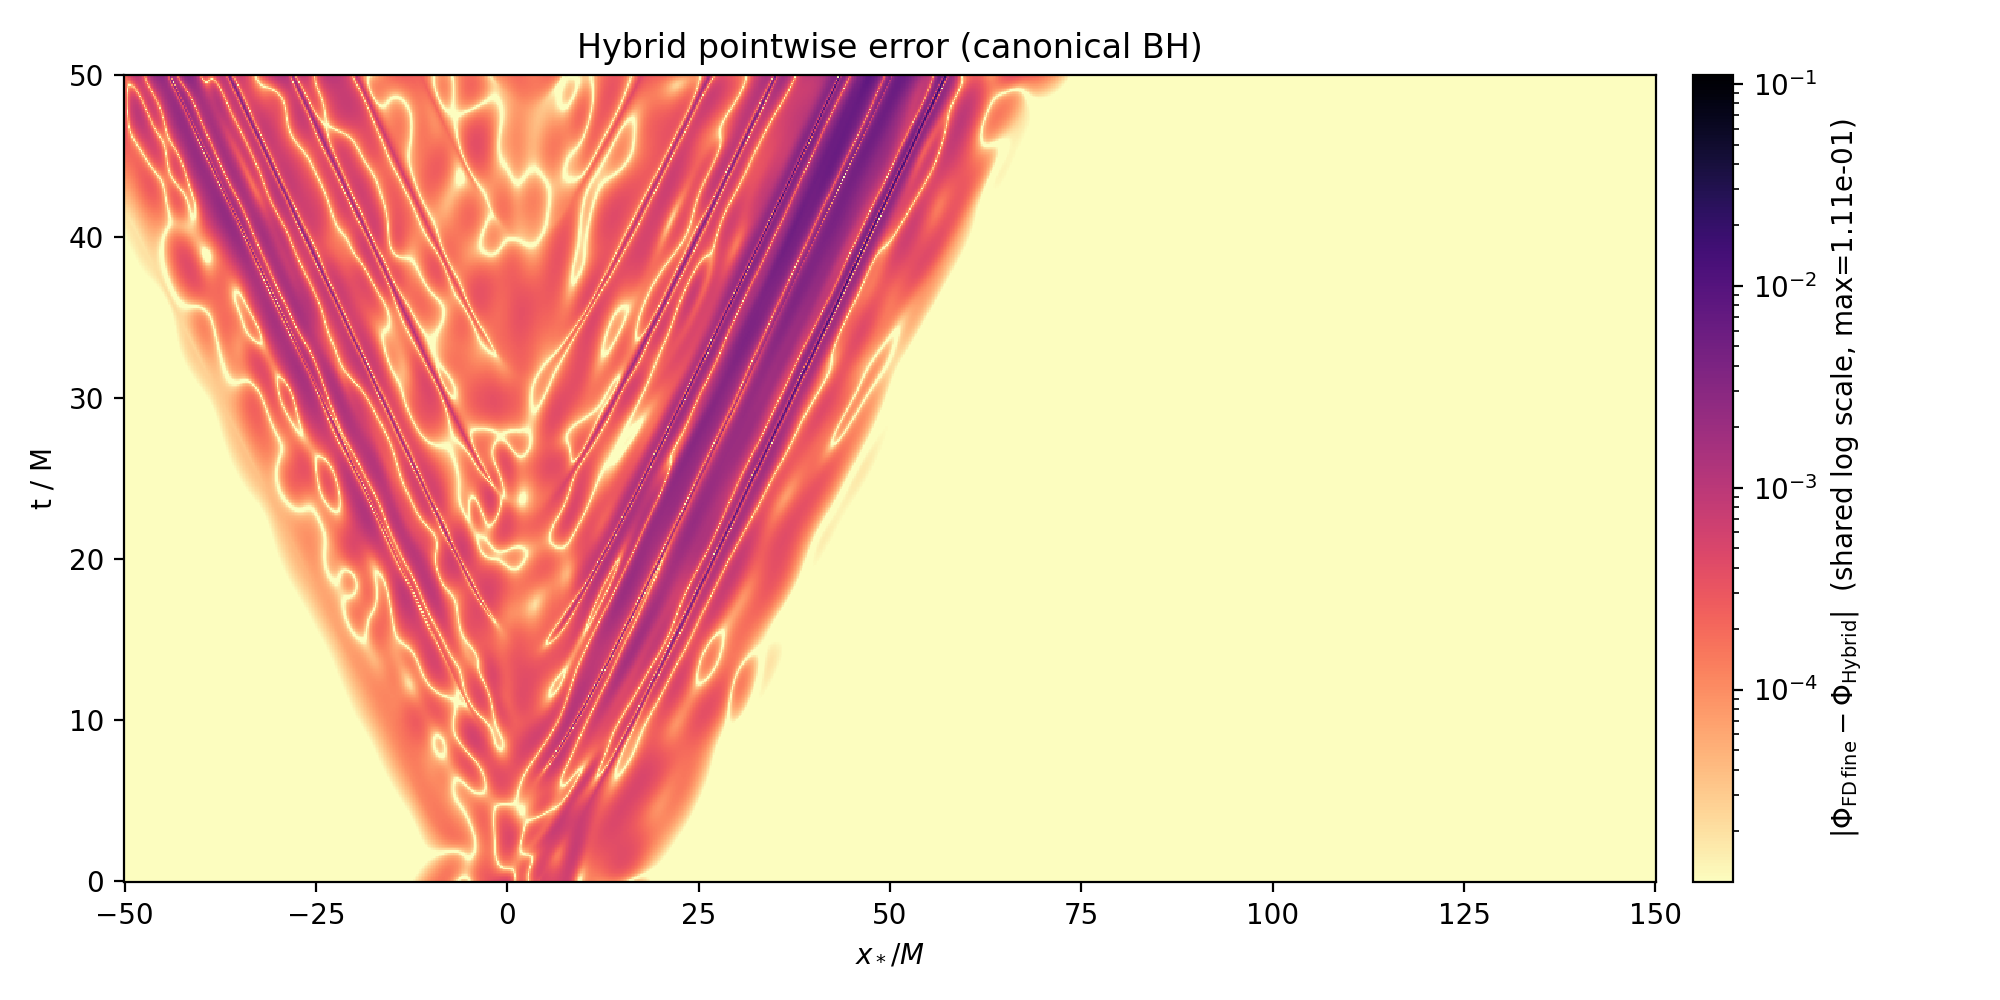
\includegraphics[width=\textwidth,height=0.46\textheight,keepaspectratio]{../outputs/hybrid/fno_sw_gate_s1em3/figs/hybrid_pointwise_error.png}
      \\{\scriptsize Pointwise error, same colour scale: coarse prior (top) vs hybrid (bottom).}
    \end{column}
    \begin{column}{0.44\textwidth}
      Error stratified by prior gradient (canonical \bh{}):
      \begin{center}\footnotesize
        \begin{tabular}{@{}lcc@{}}
          \toprule
          decile & baseline & ratio \\
          \midrule
          90--100\% (wavefronts) & $1.3\!\times\!10^{-2}$ & $\mathbf{12.3\times}$ \\
          80--90\% & $4.4\!\times\!10^{-3}$ & $9.2\times$ \\
          70--80\% & $2.2\!\times\!10^{-3}$ & $7.2\times$ \\
          $<$ median & $\sim$floor & $\sim\!1\times$ \\
          \bottomrule
        \end{tabular}
      \end{center}
      \medskip
      \begin{itemize}\small
        \item The correction tracks the gate: largest on wavefronts, vanishing in
              already-resolved regions.
        \item Over the $60.5\%$ of the domain the prior already nails, the gate holds
              network speckle to $\sim\!10^{-6}$.
      \end{itemize}
    \end{column}
  \end{columns}
\end{frame}

\begin{frame}{Hybrid FNO --- QNM extraction (median over 100 BHs)}
  \begin{center}\footnotesize
    \begin{tabular}{@{}lcccccc@{}}
      \toprule
       & \multicolumn{2}{c}{\textbf{Hybrid}} & \multicolumn{2}{c}{Coarse prior} & \multicolumn{2}{c}{Fine FD} \\
      \cmidrule(lr){2-3}\cmidrule(lr){4-5}\cmidrule(lr){6-7}
      Method & $|\Delta\omega|\%$ & $|\Delta\tau|\%$ & $|\Delta\omega|\%$ & $|\Delta\tau|\%$ & $|\Delta\omega|\%$ & $|\Delta\tau|\%$ \\
      \midrule
      M1 (FFT+log) & 0.511 & 0.394 & 0.441 & 0.324 & 0.485 & 0.262 \\
      M2 (1-mode NLS) & 0.422 & 0.818 & 0.396 & 0.860 & 0.436 & 0.805 \\
      M3 (ESPRIT) & 0.748 & 1.855 & 0.766 & 1.878 & 0.787 & 1.907 \\
      \rowcolor{green!10}
      M4 (1-D plateau) & \textbf{0.049} & 0.263 & 0.051 & 0.174 & 0.014 & 0.063 \\
      M5 (2-D plateau) & 0.052 & 0.254 & 0.051 & 0.180 & 0.014 & 0.059 \\
      \bottomrule
    \end{tabular}
  \end{center}
  \medskip
  \begin{itemize}\small
    \item \textbf{Best $\omega$: M4 at 0.049\%}; on the canonical \bh{}, M4 gives
          $\omega$ \textbf{0.045\%}, $\tau$ \textbf{0.083\%}.
    \item \textbf{Honest finding:} at a single observer the coarse prior is already at the
          extractor floor --- the hybrid is \emph{tied} with it on the \qnm{}, neither
          improving nor degrading it.
    \item \textbf{The hybrid's demonstrated value is the global field ($\sim\!10\times$)
          and generalisation}, not a single-observer \qnm{} the cheap prior already resolves.
  \end{itemize}
\end{frame}


% ══════════════════════════════════════════════════════════════════
\section{7. Overall Comparison}
% ══════════════════════════════════════════════════════════════════

\begin{frame}{Patel 2024 vs.\ our PINN vs.\ our Hybrid FNO}
  All at the \emph{identical} configuration ($\ell\!=\!2$ \zer{}, $M\!=\!1$, $x_0\!=\!4$, $\sigma\!=\!5$).
  Field error is the relative $L^2$ vs the FD reference; $\omega,\tau$ are best-of-M1--M5.
  \medskip
  \begin{center}\footnotesize
    \begin{tabular}{@{}lcccc@{}}
      \toprule
      \textbf{Model} & \textbf{field err (rel-$L^2$)} & \textbf{best $\omega$} & \textbf{best $\tau$} & \textbf{generalises?} \\
      \midrule
      Patel \emph{et al.}\ 2024 (PINN) & $28.06\%$ & $0.29\%$ (M1) & $10.25\%$ (M1) & no \\
      \textbf{Our forward PINN}        & $0.58\%$ & $\mathbf{0.029\%}$ (M4) & $1.99\%$ (M2) & no \\
      \rowcolor{green!10}
      \textbf{Our hybrid FNO}          & $0.49\%$ & $0.045\%$ (M4) & $\mathbf{0.083\%}$ (M4) & \textbf{yes} \\
      \midrule
      coarse prior (no NN) & $4.93\%$ & $0.051\%$ (M4) & $0.174\%$ (M4) & --- \\
      fine FD (truth) & --- & $0.014\%$ (M4) & $0.063\%$ (M4) & --- \\
      \bottomrule
    \end{tabular}
  \end{center}
  \medskip
  \begin{itemize}\small
    \item \textbf{Both our models crush Patel:} field $\sim\!50\times$, $\omega$ $\sim\!10\times$,
          $\tau$ by $5$--$120\times$.
    \item \textbf{$\tau$ is the discriminating quantity} --- everyone does fine on $\omega$;
          our plateau pipeline pulls $\tau$ from $\sim\!10\%$ to $\sim\!0.1\%$.
    \item \textbf{Honest:} the single-observer \qnm{} sits at the prior $+$ extractor floor
          (hybrid $\approx$ coarse prior); the hybrid's unique win is field super-resolution
          $+$ amortised generalisation.
  \end{itemize}
\end{frame}

\begin{frame}{Where each model wins}
  \begin{center}\small
    \begin{tabular}{@{}lll@{}}
      \toprule
      \textbf{Capability} & \textbf{Best model} & \textbf{Why} \\
      \midrule
      Single-config $\omega$ accuracy & forward PINN & 0.029\% via M4 plateau \\
      Damping time $\tau$ & hybrid / PINN & $\sim\!0.08\%$ (M4), $\sim\!120\times$ vs Patel \\
      Field super-resolution & \textbf{hybrid FNO} & $10\times$ over a cheap coarse solve \\
      Generalise over a family & \textbf{hybrid FNO} & one model, $1/64$ cost, no retraining \\
      QNM from coarse grid & coarse FD already & grid-robust eigenvalue \\
      \bottomrule
    \end{tabular}
  \end{center}
  \medskip
  \begin{block}{\footnotesize The take-home}
    \footnotesize
    The ringdown \emph{eigenvalue} is robust and cheap to get; the fine
    \emph{field} structure is what needs machine learning. The hybrid FNO buys
    \textbf{amortised, generalising field super-resolution} a single-instance PINN
    structurally cannot --- at a fraction of the classical cost.
  \end{block}
\end{frame}


% ══════════════════════════════════════════════════════════════════
\section{8. Future Direction --- Kerr}
% ══════════════════════════════════════════════════════════════════

\begin{frame}{Towards Kerr --- where the hybrid should pay off}
  Schwarzschild was the controlled benchmark. The hybrid is built for the regime where
  classical solves are \emph{expensive}:
  \medskip
  \begin{itemize}\small
    \item \textbf{Kerr (spinning) \bh{}s:} the \textbf{Teukolsky} equation, $2{+}1$D ---
          one extra dimension multiplies grid cost, exactly where a $1/k^{d+1}$ coarse
          prior saves most.
    \item \textbf{Spin-graded difficulty:} higher spin $\Rightarrow$ tighter light ring
          $\Rightarrow$ shorter \qnm{} wavelength $\Rightarrow$ a fixed coarse grid
          under-resolves \emph{more}. We expect the network's correction --- and its
          headroom --- to \emph{grow with spin}.
    \item \textbf{Higher multipoles ($\ell\!=\!4$):} beyond the $\ell\!=\!2$ that the
          PINN-for-QNM literature (incl.\ Patel \emph{et al.}) demonstrates.
  \end{itemize}
  \medskip
  \begin{block}{\footnotesize Status}
    \footnotesize
    Kerr corpus (mode-selective \qnm{} extraction, label-free Richardson target on a
    spin-graded coarse ladder) is \emph{in progress}; first $\ell\!=\!4$ both-axes
    (field $+$ \qnm{}) runs are queued.
  \end{block}
\end{frame}

\begin{frame}{Summary}
  \begin{enumerate}
    \item \textbf{Forward PINN:} hard BCs, gPINN, \textbf{greedy adaptive sampling},
          extended L-BFGS $\Rightarrow$ field rel-$L^2$ $0.58\%$ ($\sim\!50\times$ below
          Patel's $28\%$), $\omega$ to \textbf{0.029\%} (M4).
    \medskip
    \item \textbf{Extractors M1--M5:} plateau scans give principled, falsifiable
          $(\omega,\tau)$ with systematic-error bars; $\tau$ to $\sim\!0.1\%$.
    \medskip
    \item \textbf{Hybrid FNO:} label-free, gated coarse-FD $+$ neural-residual
          surrogate $\Rightarrow$ \textbf{$10\times$ field super-resolution} at
          $1/64$ cost, generalising across a $1000$-\bh{} family; \qnm{} preserved
          at the extractor floor.
    \medskip
    \item \textbf{Next:} Kerr / Teukolsky, where the cheap-prior saving and the
          spin-graded headroom are largest.
  \end{enumerate}
\end{frame}

\begin{frame}{}
  \begin{center}
    {\Large Thank you}
    \bigskip\\
    Questions?
  \end{center}
\end{frame}


% ══════════════════════════════════════════════════════════════════
\renewcommand{\mainend}{\inserttotalframenumber}
\makeatletter
\immediate\write\@auxout{\string\gdef\string\mainend{\the\c@framenumber}}
\makeatother

\appendix
\setbeamertemplate{footline}{%
  \hfill\usebeamerfont{footline}Appendix\hspace*{4pt}\vskip4pt%
}

\begin{frame}{Appendix --- Richardson extrapolation: derivation}
  \footnotesize
  \textbf{Setup.} A $p$-th order scheme on grid spacing $h$ admits an asymptotic error
  expansion
  \[
    \Phi^{\mathrm{c}}(h) \;=\; \Phi \;+\; C\,h^{p} \;+\; D\,h^{p+2} \;+\; \mathcal{O}(h^{p+4}),
  \]
  with $\Phi$ the exact solution and $C,D$ independent of $h$ (functions of the solution's
  derivatives). Our coarse solver is the centred 2nd-order method-of-lines scheme, so $p=2$
  and --- because centred stencils have a \emph{symmetric} truncation error --- the expansion
  runs in \emph{even} powers of $h$.
  \medskip

  \textbf{Two coarse solves} at spacings $h$ and $h/2$ (here the $k\!=\!4$ and $k\!=\!2$
  grids, ratio $2$):
  \[
    \Phi^{\mathrm{c}}(h)   = \Phi + C h^{2} + D h^4 + \mathcal{O}(h^6),
    \qquad
    \Phi^{\mathrm{c}}(h/2) = \Phi + \tfrac{C}{4} h^{2} + \tfrac{D}{16} h^4 + \mathcal{O}(h^6).
  \]
  \medskip

  \textbf{Cancel the leading error.} Seek $a\,\Phi^{\mathrm{c}}(h/2) + b\,\Phi^{\mathrm{c}}(h)$ with
  \[
    a+b = 1 \quad(\text{consistency}),
    \qquad
    a\cdot\tfrac{1}{4} + b\cdot 1 = 0 \quad(\text{kill the }h^2\text{ term})
    \;\Rightarrow\; a=\tfrac{4}{3},\; b=-\tfrac{1}{3}.
  \]
  This is the standard $p=2$ Richardson combination
  \[
    \boxed{\;\Phi^{\mathrm{R}} \;=\; \frac{4\,\Phi^{\mathrm{c}}(h/2) - \Phi^{\mathrm{c}}(h)}{3}.\;}
  \]
\end{frame}

\begin{frame}{Appendix --- Richardson: error order and use in the hybrid}
  \footnotesize
  \textbf{Residual after cancellation.} The $h^2$ term is gone by construction; the
  surviving $h^4$ term is
  \[
    \Phi^{\mathrm{R}} - \Phi
    = D\!\left(\tfrac{4}{3}\cdot\tfrac{1}{16} - \tfrac{1}{3}\right)h^4
    = D\left(\tfrac{1}{12} - \tfrac{4}{12}\right)h^4
    = -\tfrac{1}{4}D\,h^4 \;=\; \mathcal{O}(h^4),
  \]
  so two \emph{2nd-order} solves combine into a \emph{4th-order} accurate field --- without
  ever computing a finer or fine-FD solve.
  \medskip

  \textbf{Why this is the training target.} The network learns
  $\delta\Phi_{\mathrm R} = \Phi^{\mathrm R} - \Uop\Phi^{\mathrm{c}}$, a \emph{label-free}
  estimate of the coarse-prior discretisation error
  $\Phi^{\mathrm f} - \Uop\Phi^{\mathrm{c}}$, which it matches to $\mathcal{O}(h^4)$; both
  vanish as $k\to1$. The fine-FD field never enters the loss.
  \medskip

  \textbf{Assumptions (and how we honour them).}
  \begin{itemize}\itemsep1pt
    \item \emph{Asymptotic regime} --- both coarse solves resolve the same smooth solution
          (verified: Richardson cleans the QNM to $<\!0.5\%$; an aliased prior could not).
    \item \emph{Same $C$} --- identical scheme and problem at the two spacings.
    \item \emph{Upsampling must not contaminate} --- the quintic spline $\Uop$ has
          $\mathcal{O}(h^6)$ interpolation error, safely below the $\mathcal{O}(h^4)$ signal.
  \end{itemize}
\end{frame}

\begin{frame}{Appendix --- hybrid population QNM scatter}
  \centering
  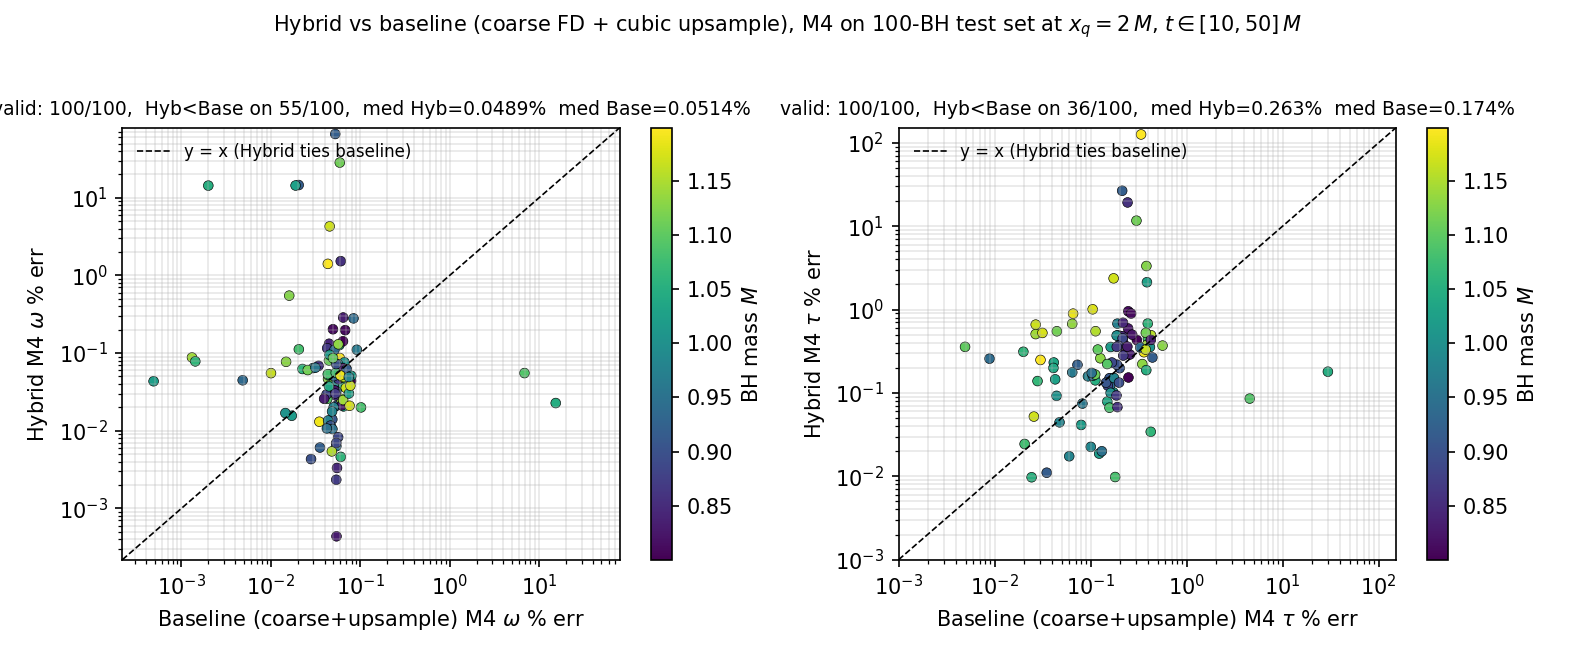
\includegraphics[width=0.7\textwidth,height=0.8\textheight,keepaspectratio]{../outputs/hybrid/fno_sw_gate_s1em3/figs/hybrid_population_scatter.png}
  \\{\footnotesize Hybrid vs coarse-prior M4 error per \bh{} ($\xq\!=\!2M$), coloured by
  mass. The bulk clusters at the joint extractor floor; outliers are ill-conditioned
  single-window fits that appear on the fine FD reference too.}
\end{frame}

\begin{frame}{Appendix --- hybrid ringdown at the observer}
  \centering
  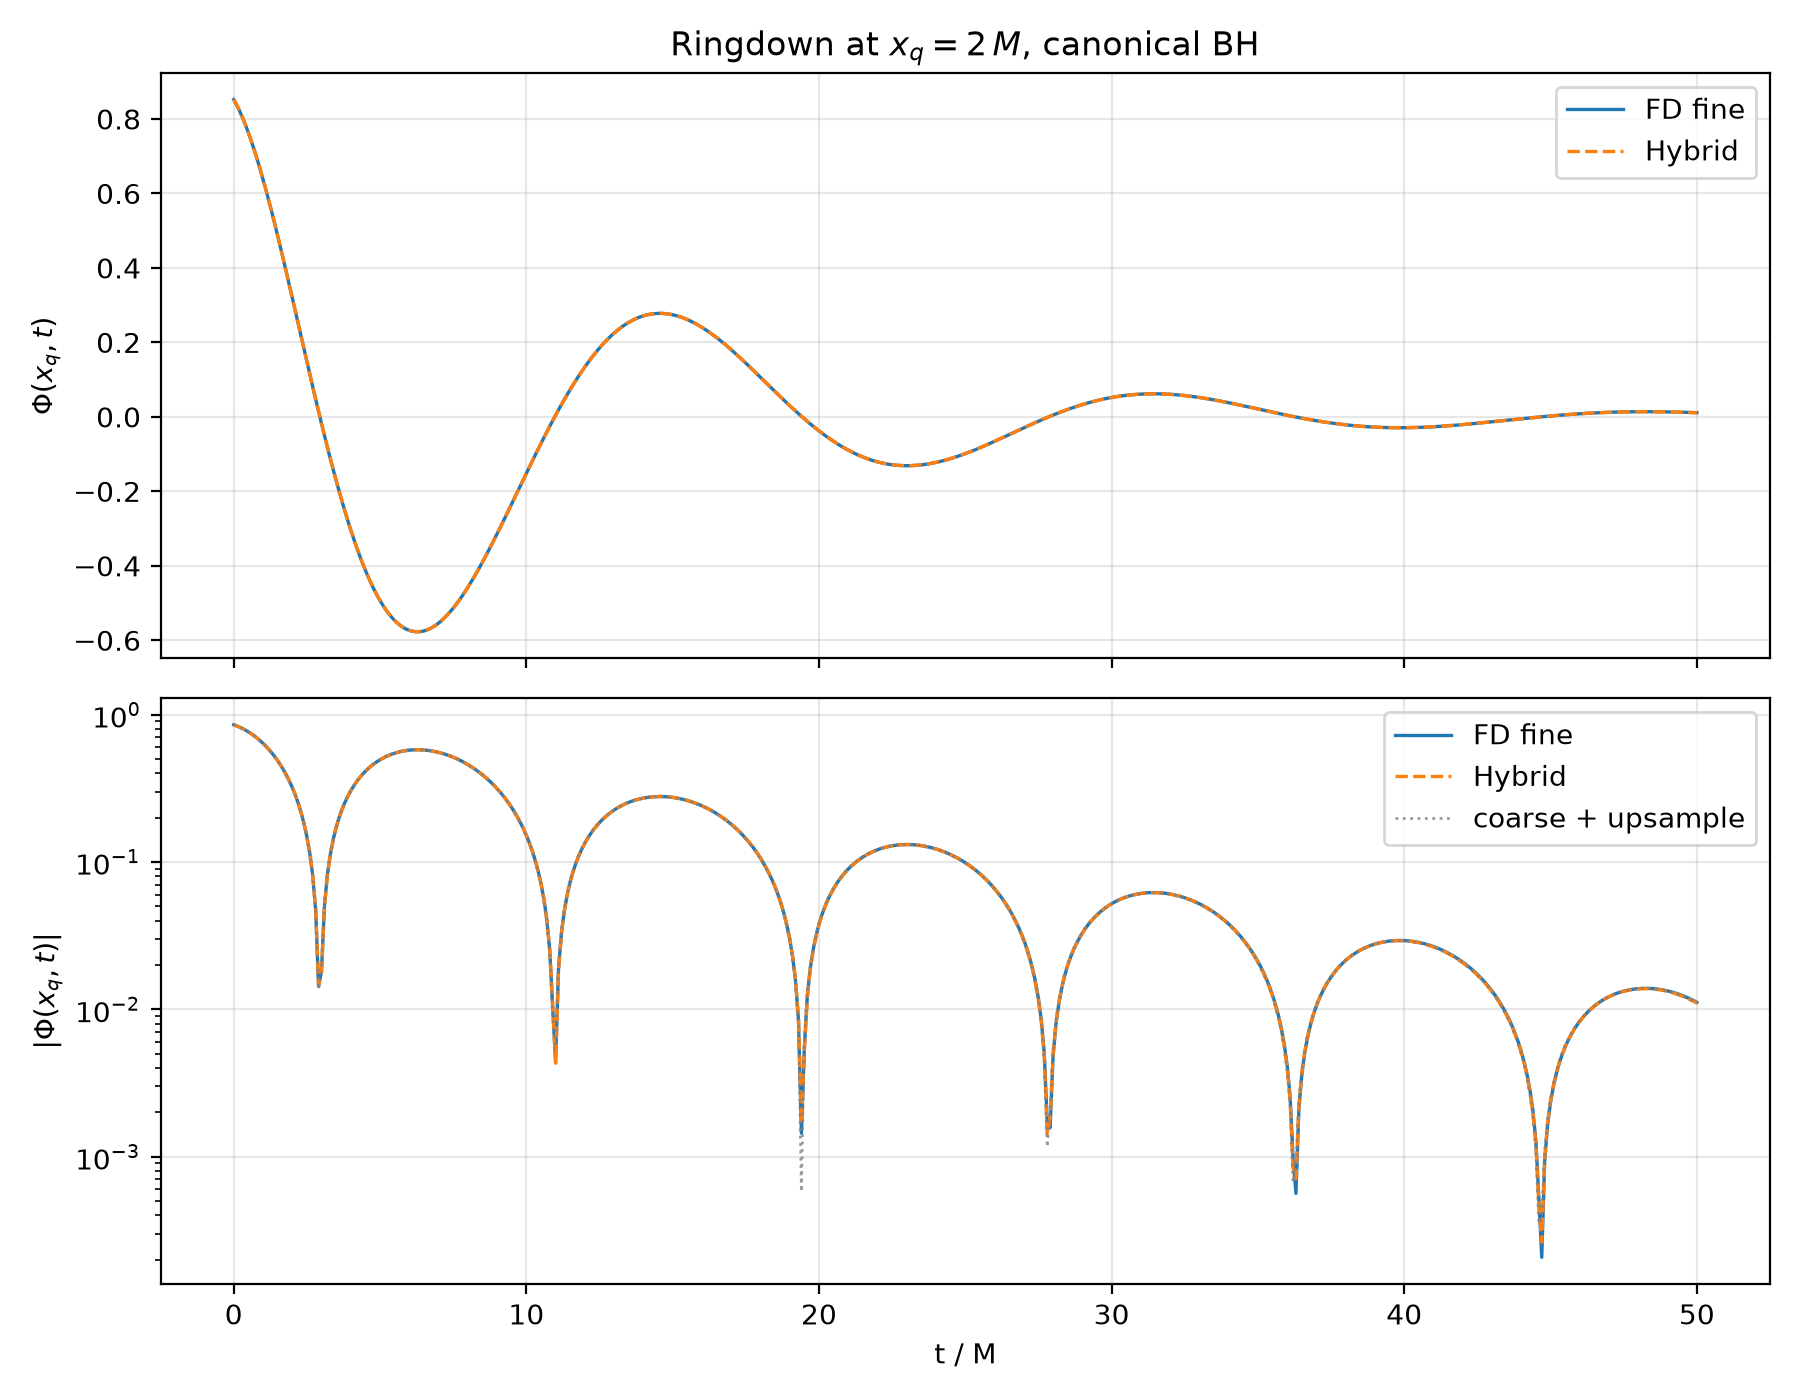
\includegraphics[width=0.7\textwidth,height=0.8\textheight,keepaspectratio]{../outputs/hybrid/fno_sw_gate_s1em3/figs/hybrid_ringdown_xq2.png}
  \\{\footnotesize $\Phi(\xq\!=\!2,t)$: fine FD (blue), hybrid (orange dashed), coarse-up
  (grey dotted) overlay to $\lesssim\!10^{-3}$ across $t\in[0,50]M$.}
\end{frame}

\end{document}
